\pdfsuppressptexinfo=-1
\pdfinfoomitdate=1
\pdftrailerid{}

\documentclass{article}

\usepackage[nonatbib]{neurips_2026} \usepackage[numbers]{natbib}


\usepackage[utf8]{inputenc}
\usepackage[T1]{fontenc}
\usepackage{hyperref}
\usepackage{url}
\usepackage{booktabs}
\usepackage{amsfonts}
\usepackage{amsmath}
\usepackage{amssymb}
\usepackage{nicefrac}
\usepackage{tikz}
\usetikzlibrary{shapes,arrows.meta,positioning,calc}
\usepackage{microtype}
\usepackage{xcolor}
\usepackage{graphicx}
\usepackage{subcaption}
\usepackage{algorithm}
\usepackage{algorithmic}
\usepackage{multirow}
\usepackage{enumitem}
\usepackage{tikz}
\usetikzlibrary{positioning, fit, arrows.meta, backgrounds, calc, shadows, shapes.geometric, shapes.misc, decorations.pathreplacing}

\newcommand{\tinker}{\textsc{Tinker}}
\newcommand{\atropos}{\textsc{Atropos}}
\newcommand{\grpo}{\textsc{Grpo}}
\newcommand{\ours}{\textsc{RL-Finetuning Bench}}

\title{Zero-Variance Fraction in GRPO: A Stratified Audit of Advantage-Collapse Diagnostics}

\author{Anonymous Author(s)\\
  Affiliation withheld for blind review\\
  \texttt{anonymous@neurips.cc}}

\newcommand{\answerPartial}[1][]{\textcolor{purple}{[Partial] #1}}

\begin{document}
\sloppy
\hbadness=10000
\vbadness=10000
\hfuzz=2pt

\maketitle

\begin{abstract}
Zero-Variance Fraction (ZVF) is a per-step sentinel for zero reward-gradient
contribution under group-relative policy advantages, not a cross-task
predictor of GRPO performance. When every rollout in a GRPO group receives
the same scalar reward, the group-relative advantage is zero and the prompt
contributes no gradient; ZVF measures the share of groups in this regime. For
binary rewards the accounting is exact:
$\operatorname{pass@}G-p^G=1-\mathrm{ZVF}$, so ZVF's complement is
contrastive group yield rather than an independent performance statistic.
We make two paired claims about how to use this quantity. \emph{Positive:}
per-step ZVF (and its complement $\mathrm{GU}_t = 1-\mathrm{ZVF}_t$) is a
mechanically interpretable online utilization meter that, paired with batch
reward mean, distinguishes all-wrong collapse from all-correct saturation
and from informative-contrast training; we demonstrate this with tool-use
runs that sit at $\mathrm{ZVF}{=}1$, $\mathrm{GU}{=}0$, reward $0$ from
step~1 (Qwen3-32B and Llama-3.1-8B), contrasted with a GSM8K run whose
GU and reward both move. \emph{Negative:} the pooled cross-task ZVF--reward
correlation that earlier drafts (and concurrent work) cite as evidence that
ZVF predicts GRPO outcomes does \emph{not} survive within-task
stratification ($r{=}-0.769$, $p{=}0.0008$, $N{=}15$ pooled $\to$ $r{=}+0.40$,
$p{=}0.09$, $N{=}19$ within-GSM8K; $r{=}+0.13$, $N{=}7$ model-varying); it is
confounded by task identity. We audit pooled correlations under stratification
and partial-correlation controls and provide a regime-to-action triage table.
We release step-level ZVF/GU traces, formalization, and analysis code at
\url{https://anonymous.4open.science/r/agentic-grpo-bench-anon-2C6B}.
\end{abstract}
 
\begin{figure}[htbp]
\centering
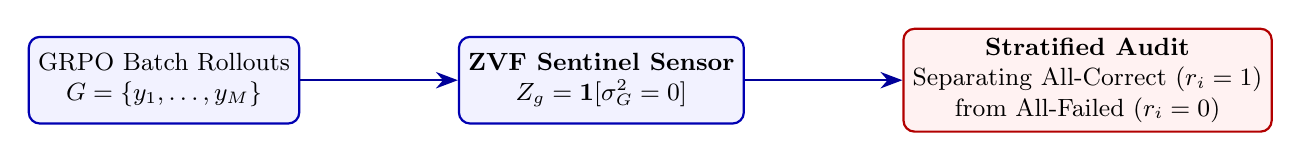
\begin{tikzpicture}[
    node distance=1.5cm and 2.0cm,
    block/.style={rectangle, draw=blue!70!black, fill=blue!5, thick, rounded corners, align=center, minimum height=1.1cm, minimum width=3.2cm, font=\small},
    audit/.style={rectangle, draw=red!70!black, fill=red!5, thick, rounded corners, align=center, minimum height=1.1cm, minimum width=3.4cm, font=\small},
    arrow/.style={-{Stealth[scale=1.2]}, thick, draw=blue!60!black}
]
    \node [block] (grpo) {GRPO Batch Rollouts\\$G = \{y_1, \dots, y_M\}$};
    \node [block, right=of grpo] (sentinel) {\textbf{ZVF Sentinel Sensor}\\$Z_g = \mathbf{1}[\sigma_G^2 = 0]$};
    \node [audit, right=of sentinel] (strat) {\textbf{Stratified Audit}\\Separating All-Correct ($r_i=1$)\\from All-Failed ($r_i=0$)};

    \draw [arrow] (grpo) -- (sentinel);
    \draw [arrow] (sentinel) -- (strat);
\end{tikzpicture}
\caption{\textbf{ZVF Sentinel Diagnostic \& Task-Stratification Architecture (R02).} Monitoring online zero-variance events and stratifying prompt difficulty.}
\label{fig:zvf_sentinel_architecture}
\end{figure}

\section{Introduction}
\label{sec:intro}

Group-relative policy optimization (GRPO) and its descendants now underlie a
large fraction of recent reasoning-RL pipelines~\citep{shao2024deepseekmath,guo2025deepseekr1nature}, replacing the value-function critic of
PPO~\citep{schulman2017proximal} with a leave-one-out advantage computed
within a small group of rollouts that share a prompt. Because the advantage
is the within-group reward minus the within-group mean (or median),
\emph{any group in which all rollouts receive identical rewards contributes a
zero advantage to every token} and therefore zero gradient. We call the
share of such groups in a training batch the \textbf{Zero-Variance Fraction}
(ZVF).

\paragraph{ZVF is a per-step sentinel, not a cross-task predictor.}
The framing we adopt in this paper is narrow and mechanical. At step~$t$,
$\mathrm{ZVF}_t = 1$ implies that every rollout group in the batch has zero
reward variance and therefore zero reward-gradient contribution; the
complementary $\mathrm{GU}_t = 1-\mathrm{ZVF}_t$ is an online \emph{utilization
meter} for the reward channel of the GRPO update. Pairing $\mathrm{ZVF}_t$
with batch reward mean separates all-wrong collapse ($\mathrm{ZVF}{\approx}1$,
mean reward $\approx 0$) from all-correct saturation ($\mathrm{ZVF}{\approx}1$,
mean reward $\approx 1$) from informative-contrast training
($\mathrm{ZVF}{<}1$, intermediate mean reward). This is the regime in which
ZVF is genuinely useful as instrumentation, and it is what caught the
sparse-reward tool-use failures in our benchmark, where every Tinker run
sat at $\mathrm{ZVF}{=}1$ from step~1 (Section~\ref{sec:zvf-analysis},
Figure~\ref{fig:zvf-sentinel}).

\paragraph{The pooled cross-task correlation is task identity in disguise.}
Earlier drafts of this paper, and several concurrent ``GRPO failure-mode''
analyses, summarized ZVF by pooling across tasks and computing a single
correlation between mean ZVF and final reward. Across the 15 cross-task
runs reported in earlier drafts, mean ZVF and last-10 reward correlate at
Pearson $r{=}-0.769$ ($p{=}0.0008$). On a larger $N{=}29$ sample with
released step-level traces, the pooled correlation drops to $r{=}-0.44$.
\emph{Both numbers are dominated by task identity, not by GRPO dynamics:}
tool-use runs sit at $\mathrm{ZVF}{\approx}1$ and reward $0$, GSM8K runs
sit at $\mathrm{ZVF}{\approx}0.085$ and reward $0.3$--$0.9$. Stratifying
within GSM8K, the correlation flips sign to $r{=}+0.40$ ($p{=}0.09$,
$N{=}19$); restricting to the seven GSM8K runs that vary model rather than
hyperparameter, $r{=}+0.13$ ($p{=}0.79$). The ``ZVF predicts performance''
story disappears under stratification and partial-correlation controls
(Section~\ref{sec:zvf-analysis}, Table~\ref{tab:evidence-grade}).

\paragraph{This paper is a focused statistical audit.}
We do not propose a new GRPO algorithm and we do not propose ZVF as a
benchmark scoring statistic. We make two paired claims and audit them. The
positive claim is that per-step ZVF inside a single task is a useful
zero-gradient sentinel and utilization meter; we provide a triage table
mapping (ZVF, reward) regimes to suggested actions. The negative claim is
that the pooled cross-task ZVF--reward correlation cited in earlier drafts
and concurrent work is confounded by task identity, does not survive
within-task stratification, and should not be used to rank GRPO runs.

This main-track paper is the focused sentinel/stratification claim in the larger
program. The adaptive controller and the GRPO--PPO--SAO unification are companion
proposals and do not upgrade the evidence reported here.

\paragraph{Contributions.}
(i)~A clean formalization of ZVF and its mechanical coupling to group size
and baseline accuracy under group-relative advantage estimators
(Section~\ref{sec:zvf-analysis} and Appendix~\ref{sec:appendix:zvf-formalization}).
(ii)~A positive sentinel demonstration on tool-use runs (Qwen3-32B and
Llama-3.1-8B, $\mathrm{ZVF}{=}1$, $\mathrm{GU}{=}0$, reward $0$ from step~1)
contrasted with a GSM8K run whose GU and reward both move, plus a triage
table mapping (regime, ZVF, reward) to action
(Section~\ref{sec:zvf-analysis}).
(iii)~A stratified audit of the pooled cross-task ZVF--reward correlation:
the pooled $r{=}-0.769$ collapses under within-task stratification on
GSM8K to a non-significant, sign-flipped $r{=}+0.40$ (and $r{=}+0.13$,
$N{=}7$ model-varying); we read this as a methodological warning, not a
defeat of the mechanical claim.
(iv)~A cross-stack benchmark of step-level ZVF traces on 79 GRPO runs across
7 RL libraries, 5 model families, and total parameter scales 0.6B--671B
(active 0.6B--37B for the largest mixture-of-experts checkpoints), released
as an artifact rather than headlined as a benchmark contribution
(Appendix~\ref{sec:run-manifest}).
(v)~Released step-level ZVF/GU traces, formalization, and reanalysis code.
 


\section{Related Work}
\label{sec:related}

\ours{} sits at the intersection of policy-gradient post-training for
language models, reasoning supervision, tool-use agents, scaling analyses, and
benchmark reproducibility. We use this section to define the context for our
measurements. Where concurrent work studies the same within-group
zero-variance phenomenon that motivates our ZVF diagnostic, we cite it as
mechanism corroboration; we do not claim those papers independently validate
our specific numerical ZVF results, nor do we use them as evidence for any
projected variance-mitigation row.

\subsection{RL Algorithms for Large Language Models}
\label{sec:related:algos}

Proximal Policy Optimization (PPO)~\cite{schulman2017proximal} remains the
standard reference point for RLHF-style post-training, including
InstructGPT-style systems~\cite{ouyang2022training, christiano2017deeprlhf,
stiennon2020summarize, bai2022hhrlhf, bai2022claudecai}. Direct Preference
Optimization (DPO)~\cite{rafailov2024direct} reframed preference learning as a
classification objective and motivated RL-free baselines such as
IPO~\cite{azar2024ipo}, KTO~\cite{ethayarajh2024kto},
SimPO~\cite{meng2024simpo}, ORPO~\cite{hong2024orpo}, and
SLiC~\cite{zhao2023slic}. Our benchmark includes no-rollout baselines to keep
the distinction between sampled policy-gradient training and preference
classification explicit.

Group Relative Policy Optimization (GRPO) was introduced with
DeepSeekMath~\cite{shao2024deepseekmath} and popularized by
DeepSeek-R1~\cite{guo2025deepseekr1, guo2025deepseekr1nature}. Subsequent
public GRPO-family work studies known implementation sensitivities rather than
establishing our measurements. Dr.~GRPO~\cite{tong2025drgrpo} analyzes length
and difficulty biases in the standard objective. GSPO~\cite{qwen2025gspo},
DAPO~\cite{yu2025dapo}, and VAPO~\cite{bytedance2025vapo} are useful context
for production-scale sequence-level and large-batch reasoning RL. Back to
Basics~\cite{ahmadian2024backtobasics} shows that carefully implemented
REINFORCE-style methods can remain competitive. These works motivate the
implementation and diagnostic axes we measure; they are not used as evidence
for any numerical result in \ours{}.

\subsection{Concurrent Zero-Variance Work}
\label{sec:related:concurrent-zv}

A cluster of 2025--2026 GRPO-family papers independently identifies the same
within-group zero-variance failure mode that motivates our Zero-Variance
Fraction (ZVF) diagnostic: when every rollout in a group receives the same
scalar reward, the group-relative advantage vanishes and no gradient signal
reaches the policy. NGRPO~\cite{nan2025ngrpo} formalizes the case as
``homogeneously correct or incorrect'' groups and proposes advantage
calibration with a hypothesised maximum-reward virtual sample plus asymmetric
clipping. RL-ZVP~\cite{le2025rlzvp} (ICLR 2026) names the construct
\emph{zero-variance prompts} and shows that entropy-guided advantage shaping
on such prompts yields up to $+8.61$ accuracy points across six math
benchmarks over standard GRPO. Scaf-GRPO~\cite{zhang2025scaffgrpo} frames the
same phenomenon as a ``learning cliff'' where problems beyond model capability
collapse to zero reward and zero advantage, and counters it with tiered
in-prompt scaffolds. LENS~\cite{feng2025lens} addresses the all-wrong-group
sub-case via confidence-reweighted penalties on negative rollouts. Hard
Examples~\cite{pikus2025hardexamples} treats zero-variance saturation as the
fundamental annotation-budget bottleneck and shows that training on the
hardest examples reduces it. EBPO~\cite{han2026ebpo} proposes an empirical
Bayes shrinkage estimator that guarantees a non-vanishing gradient even in
saturated-failure regimes.

We cite these works narrowly. They corroborate the existence and importance of
the within-group zero-variance failure mode, and one of them (RL-ZVP) is at a
peer-reviewed venue. They do \emph{not} validate our specific quantitative
ZVF results -- the project's correlation $\rho$ values, step-25 to step-100
stress-test predictiveness, or any cross-task ZVF threshold -- which remain
internal-artifact diagnostics computed from our rollout traces. We make no
priority claim with respect to these papers, several of which were submitted
before our ZVF traces were complete; we are rigorous, not first.

 
\section{Experimental Setup}
\label{sec:setup}

We instrument GRPO-style training with step-level group reward statistics
across 79 runs spanning 7 RL libraries and the Qwen3, Qwen3.5, and Llama-3.x
model families at scales from $0.6$B to $671$B total parameters
($0.6$B--$37$B active for the largest MoE checkpoints). ZVF is computed per
training step as the fraction of rollout groups whose reward variance is
exactly zero; full per-library code paths are listed in
Appendix~\ref{sec:appendix:zvf-pipeline}. Headline experiments use Qwen3-8B with
LoRA rank 32, Adam ($\beta_1{=}0.9$, $\beta_2{=}0.95$), learning rate
$10^{-4}$, and 5 seeds in $\{42,123,456,789,1024\}$. Frontier-scale runs are
single-seed and reported as case studies. Reproducibility,
limitations, and ethics are deferred to
Appendix~\ref{sec:appendix:reproducibility},
Appendix~\ref{sec:appendix:limitations}, and
Appendix~\ref{sec:appendix:ethics}; auxiliary reward-trajectory instability
signals are deferred to Appendix~\ref{sec:appendix:instability}.

\section{Zero-Variance Fraction: A Stratified Audit}
\label{sec:results}


\subsection{Per-step sentinel framing}
\label{sec:zvf-sentinel}


\textbf{Zero-Variance Fraction (ZVF)} at step $t$ is the fraction of prompts
for which all $G$ completions receive identical rewards:
\[
  \mathrm{ZVF}_t = \frac{1}{|\mathcal{P}_t|}\sum_{p \in \mathcal{P}_t}
  \mathbf{1}\bigl[\operatorname{Var}_{c \sim \mathcal{C}(p)}\,r(c) = 0\bigr].
\]
When $\mathrm{ZVF}_t = 1$, every prompt contributes zero gradient.
\textbf{Gradient Utilization} $\mathrm{GU}_t = 1 - \mathrm{ZVF}_t$ measures
the fraction of prompts providing informative signal. The two quantities
together with batch reward mean separate three operationally distinct
regimes: \emph{all-wrong collapse} ($\mathrm{ZVF}{\approx}1$, reward $\approx
0$), \emph{all-correct saturation} ($\mathrm{ZVF}{\approx}1$, reward $\approx
1$), and \emph{informative contrast} ($\mathrm{ZVF}{<}1$, intermediate
reward). The mechanical claim is that whenever
$\mathrm{ZVF}_t = 1$, the reward channel of the GRPO advantage estimator
contributes nothing to that step's gradient
(formal statement and proof in
Appendix~\ref{sec:appendix:zvf-formalization}).

\paragraph{Positive demonstration: tool-use as the all-wrong-collapse regime.}
Figure~\ref{fig:zvf-sentinel} shows the sentinel in operation. Two
single-seed Tinker tool-use runs (Qwen3-32B and Llama-3.1-8B,
shaped reward, $G{=}8$, 30 steps) sit at $\mathrm{ZVF}_t = 1$
from step~1 onward (panel a) while the batch reward mean stays at $0$
(panel b): GU is identically zero, the reward channel contributes
nothing, and the entire 30-step training run is mechanically a no-op.
A contrasting Wave-6 GSM8K ablation cell on Qwen3-8B (panel c, twin axes)
shows the informative-contrast regime: ZVF oscillates between $0$ and $1$
while the batch reward mean varies between roughly $0$ and $0.8$. Pairing
the two telemetry channels diagnoses the tool-use task as a reward-design
failure (no within-group contrast at any step) without inspecting any
reward curve in isolation. Table~\ref{tab:zvf-triage} records the suggested
operational action in each regime.

\begin{figure}[t]
\centering

\includegraphics[width=\linewidth]{figures/v2/zvf_sentinel.png}
\caption{\textbf{ZVF as a per-step zero-gradient sentinel.}
\textbf{(a)}~Tool-use ZVF traces for Qwen3-32B/tool\_use and
Llama-3.1-8B/tool\_use sit at $\mathrm{ZVF}_t = 1$ from step~1 onward
(persistent zero-gradient sentinel). \textbf{(b)}~Tool-use batch reward mean
remains at $0$ for the same runs ($\mathrm{GU}_t = 0$, all-wrong-collapse
regime). \textbf{(c)}~A representative Wave-6 GSM8K ablation cell on
Qwen3-8B (temperature $0.4$, rank $32$, batch $2$) shows the
informative-contrast regime on the same instrumentation: ZVF (vermillion,
left axis) oscillates while the batch reward mean (green, right axis,
twin) varies between $\sim 0$ and $\sim 0.8$. Pairing $\mathrm{ZVF}_t$
with batch reward mean separates collapse from saturation from
informative contrast (Table~\ref{tab:zvf-triage}); single-seed Tinker
case studies, no error bars.}
\label{fig:zvf-sentinel}
\end{figure}

\begin{table}[t]
\centering\small
\setlength{\tabcolsep}{5pt}
\begin{tabular}{p{0.22\linewidth}cp{0.13\linewidth}p{0.27\linewidth}p{0.20\linewidth}}
\toprule
\textbf{Regime} & \textbf{ZVF} & \textbf{Reward mean} & \textbf{Interpretation} & \textbf{Action} \\
\midrule
All-wrong collapse & $\sim$1 & $\sim$0 &
zero reward-gradient; task / reward too hard &
redesign reward / curriculum \\
All-correct saturation & $\sim$1 & $\sim$1 &
zero reward-gradient; task solved &
stop or increase difficulty \\
Useful contrast & $<$1 & intermediate &
informative groups exist &
continue training \\
Cross-task pooled signal & mixed & mixed &
confounded by task identity &
do not rank runs \\
\bottomrule
\end{tabular}
\caption{Triage table mapping (ZVF, reward) regimes to suggested
operational action. The first three rows describe per-step in-task
diagnoses for which $\mathrm{ZVF}_t$ is genuinely informative; the last
row describes the pooled cross-task setting in which ZVF should
\emph{not} be used to rank runs (Section~\ref{sec:zvf-stratification}).}
\label{tab:zvf-triage}
\end{table}

\subsection{Stratified audit of the pooled cross-task correlation}
\label{sec:zvf-stratification}
\label{sec:zvf-analysis}


\paragraph{Headline empirical result: the pooled correlation does not
survive stratification.}
We tested whether mean ZVF predicts last-10 reward across our cross-stack
benchmark. The pooled cross-task correlation is large ($r_{\text{Pearson}}
= -0.769$, $p = 0.0008$ on the original $N{=}15$ sample;
$r_{\text{Pearson}} = -0.44$ on the larger $N{=}29$ sample of runs with
released step-level traces in our artifact). \textbf{Both pooled numbers
are dominated by task identity, not by GRPO dynamics.} Tool-use experiments
sit at $\mathrm{ZVF} = 100\%$ at $\sim$0\% reward; GSM8K experiments
average $\mathrm{ZVF} = 8.5\%$ at much higher reward. Stratifying within
GSM8K, the apparent monotone relationship disappears and flips sign:
Pearson $r = +0.40$ ($p = 0.09$, $N{=}19$ Tinker GSM8K runs spanning 5
model families and the Wave-6 Qwen3-8B hyperparameter ablation), Spearman
$\rho = +0.28$ ($p = 0.24$). Restricted to the seven Tinker GSM8K runs that
vary model rather than hyperparameter (Qwen3-8B, Qwen3.5-4B,
Llama-3.1-8B, GPT-OSS-20B, Kimi-K2, DeepSeek-V3.1, Nemotron-120B), the
within-task Pearson is $r = +0.13$ ($p = 0.79$, $N{=}7$).

The implication is prescriptive. The ``ZVF predicts performance'' story
holds only if one is willing to credit it for the task-identity gap
between tool-use ($\mathrm{ZVF}{=}1$, reward $0$) and GSM8K
($\mathrm{ZVF}{=}0.085$, reward $0.3$--$0.9$). Inside a homogeneous task,
ZVF does not rank GRPO runs in our data. Cross-task pooled ZVF
correlations should therefore not be cited as evidence that ZVF predicts
GRPO failure; they primarily report which tasks the rollouts were drawn
from.

\section*{Stratified Diagnostics}
\label{sec:stratified-diagnostics}

\paragraph{Bootstrap CIs and permutation tests.}
Pearson $r$ between mean ZVF and last-10 reward on each of the four cell-pools
used in this paper, with 10\,000-resample bootstrap 95\% CIs and
10\,000-permutation $p$-values (Table~\ref{tab:zvf-bootstrap}). The pooled
cross-task signal is large; the within-task subsets cross zero.

\begin{table}[h]
\centering\small
\begin{tabular}{lrrrr}
\toprule
Analysis & $r$ & $N$ & 95\% CI (bootstrap) & $p_{\text{perm}}$ \\
\midrule
Pooled original                 & $-0.769$ & $15$ & $[-0.93,\,-0.52]$ & $0.0004$ \\
Pooled extended                  & $-0.443$ & $29$ & $[-0.69,\,+0.03]$ & $0.0146$ \\
Within GSM8K                    & $+0.401$ & $19$ & $[-0.08,\,+0.83]$ & $0.0837$ \\
GSM8K model-varying\textsuperscript{\dag}    & $+0.126$ & $7$  & $[-0.97,\,+1.00]$ & $0.8139$ \\
\bottomrule
\end{tabular}
\caption{ZVF--last-10 reward correlations with bootstrap CIs and permutation
$p$-values. The extended pool reports every cell whose step-level ZVF trace is
in the released artifact. \textsuperscript{\dag}~The $N{=}7$ nonparametric CI
is uninformative; the parametric Fisher-$z$ CI is $[-0.69,\,+0.80]$, also
crossing zero.}
\label{tab:zvf-bootstrap}
\end{table}

\paragraph{Partial correlations.}
With task fixed effects, log group size, and pre-RL accuracy as controls
(Table~\ref{tab:zvf-partials}); we never control for last-10 reward, the
outcome. Adding task FE alone collapses the pooled $r$ from $-0.44$ to
$-0.03$; with any combination of $\log G$ and base accuracy the partial $r$
is between $+0.02$ and $+0.14$ and never significant.

\begin{table}[h]
\centering\small
\begin{tabular}{lrrrl}
\toprule
Specification & $r_{\text{partial}}$ & df & $p$ & Interpretation \\
\midrule
Raw pooled, no controls                          & $-0.443$ & $27$ & $0.016$ & Task is a lurking variable. \\
$+$~task FE                                      & $-0.026$ & $26$ & $0.896$ & Task identity removes the sign. \\
GSM8K within-task                                & $+0.401$ & $17$ & $0.088$ & Sign flips, CI crosses zero. \\
GSM8K model-varying                              & $+0.126$ & $5$  & $0.788$ & Underpowered ($N{=}7$). \\
Pooled $+$ task FE $+$ $\log G$                  & $+0.021$ & $25$ & $0.916$ & Group size does not rescue it. \\
Pooled $+$ task FE $+$ base acc                  & $+0.135$ & $25$ & $0.502$ & Pre-RL ability does not rescue it. \\
Pooled $+$ task FE $+$ $\log G$ $+$ base acc     & $+0.136$ & $24$ & $0.507$ & Joint controls; not significant. \\
GSM8K $+$ $\log G$ $+$ base acc                  & $+0.420$ & $15$ & $0.094$ & Within-task partial agrees with raw. \\
\bottomrule
\end{tabular}
\caption{Partial Pearson correlations of mean ZVF with last-10 reward
(\texttt{pingouin.partial\_corr}). Last-10 reward is the outcome and is never
on the right-hand side. Stack fixed effects are not reported (too little
within-stack variation: $\le 3$ stacks with $\ge 2$ runs).}
\label{tab:zvf-partials}
\end{table}

\paragraph{Interpretation.}
The pooled correlation does not survive stratification: with task fixed
effects $r$ collapses to $-0.03$, and on the largest within-task subset the
sign flips to $+0.40$. The remaining within-GSM8K signal is underpowered,
with a 95\% CI that crosses zero. This is not evidence of absence---it is
evidence that the pooled monotone story is not supported once the task
confound is removed.
 
\paragraph{Auxiliary statistics.}
Model scale does not uniformly reduce ZVF
($r_\text{Pearson} = -0.257$). A one-way ANOVA across model families
yields $F(4,10) = 0.949$, $p = 0.476$, which does not resolve family-level
differences in this mixed task/model sample. We retain these auxiliary
statistics in the artifact for completeness; they should not be read as
contradicting the stratified within-task null.

\begin{figure}[htbp]
\centering

\includegraphics[width=\textwidth]{../figures/v2/zvf_correlation}
\caption{\textbf{Left:} Pooled ZVF vs.\ final performance scatter
($r = -0.769$, $p = 0.0008$, $N{=}15$). The apparent strong negative
correlation is task-confounded: the upper-right tool-use cluster sits at
$\mathrm{ZVF}{=}1$, reward $0$; the lower-left GSM8K cluster sits at
$\mathrm{ZVF}{\le}0.5$, reward $\geq 0.3$. \textbf{Right:} Mean ZVF by
model family. Llama's high mean ZVF is driven entirely by tool-use
experiments. Within-GSM8K stratified Pearson is $r = +0.40$ ($p = 0.09$,
$N{=}19$); restricted to model-varying GSM8K, $r = +0.13$ ($p = 0.79$,
$N{=}7$). The pooled negative correlation in this scatter does not
survive stratification.}
\label{fig:zvf-correlation}
\end{figure}

\subsection{Group size enters ZVF mechanically; it does not rescue the pooled story}
\label{sec:grpo-dpo}


ZVF is mechanically coupled to group size $G$ and per-prompt accuracy $p$
under binary outcome rewards:
$\mathrm{ZVF}(p, G) = p^G + (1-p)^G$, so
$\mathrm{GU}(p, G) = 1 - p^G - (1-p)^G$. Beyond $G{=}8$, the marginal GU
gain from larger groups approaches zero for moderate accuracies $p \in
[0.2, 0.8]$ (the gain from $G{=}16 \to G{=}32$ is less than $0.3\%$ at
$p{=}0.5$). Empirically, in the single-seed Wave-2 Qwen3-8B/GSM8K sweep
the fixed-step last-10 reward is non-monotone in $G$
($G{=}4{:}\,0.52$, $G{=}32{:}\,0.44$, $G{=}16{:}\,0.38$, $G{=}2{:}\,0.38$,
$G{=}8{:}\,0.34$); a token-budget-normalized reanalysis
(Appendix~\ref{sec:appendix:group-size-reconcile}) shifts the inverted-U
apex rightward with total tokens $T$, so neither $G{=}4$ nor $G{=}32$ is
a universal optimum. We mention $G$ only because it is mechanically tied
to $\mathrm{ZVF}(p,G)$; $G$ does not rescue the pooled cross-task story.

A two-seed matched-budget panel (E-R2b: 2{,}560 rollouts per arm,
$G{=}2\times160$ steps vs.\ $G{=}16\times20$ steps, LoRA rank 4, 512-token
completions, seeds 123/456) sharpens the mechanical coupling into a
trajectory claim: the $G{=}2$ arms (160 steps) drive train reward to
$\approx0.9$--$1.0$ on the sampled pool and end in sustained
$\mathrm{ZVF}\approx0.75$--$1.0$ --- all-\emph{correct} groups, the
high-$p$ zero-variance wall that $\mathrm{ZVF}(p,G)=p^G+(1-p)^G$ predicts
as $p\to1$ --- while the $G{=}16$ arms (20 steps at the same budget) end
mid-learning at train reward $\approx0.3$--$0.5$ with $\mathrm{ZVF}$ at
$0$--$0.25$ throughout. Small $G$ converts a fixed rollout budget into more optimizer
steps early, then exhausts its own gradient signal in the endgame
(Tier~C, two seeds per arm).

\paragraph{Loss form leaves no ZVF signature at this scale.} A six-arm
uncapped panel (1{,}024-token completions, $G{=}8$, batch 4, 30 steps,
three seeds per loss) comparing GRPO with Dr.GRPO's $/\sigma$-free
advantage found no length inflation in \emph{either} loss --- mean
completion length declines 3.8--12.2\% in all six arms --- and no late-ZVF
separation (Dr.GRPO 0.45/0.70/0.72 vs.\ GRPO 0.47/0.47/0.55). Whatever
Dr.GRPO's normalization change does at larger scale, it has no observable
ZVF or length footprint on Qwen3-8B/GSM8K (Tier~C, $n{=}3$ seeds per
loss).

\subsection{Evidence Grade of Each Claim}
\label{sec:evidence-grade}
This paper mixes claims at very different levels of statistical strength.
Table~\ref{tab:evidence-grade} segregates every quantitative claim in the
main text by evidence grade so that downstream readers do not have to
reconstruct it from scattered caveats. The two rows we ask readers to take
away are the headline claims at the top of the table; the rest are
auxiliary or descriptive.

\begin{table}[htbp]
\centering\small
\setlength{\tabcolsep}{4pt}
\begin{tabular}{p{0.42\linewidth}p{0.18\linewidth}p{0.32\linewidth}}
\toprule
\textbf{Claim} & \textbf{Grade} & \textbf{Notes} \\
\midrule
\multicolumn{3}{l}{\textit{Headline claims (paper's main contributions)}} \\
\midrule
ZVF $\to$ zero gradient under GRPO is mechanical &
A (definitional) &
Appendix~\ref{sec:appendix:zvf-pipeline}. \\
\textbf{Per-step ZVF + reward mean is a sentinel that distinguishes
all-wrong collapse, all-correct saturation, and informative contrast} &
A (mechanical / case study) &
Figure~\ref{fig:zvf-sentinel}, Table~\ref{tab:zvf-triage}; tool-use
demonstration is single-seed Tinker. \\
\textbf{The pooled cross-task ZVF--performance correlation does not
survive within-task stratification on GSM8K
($r{=}+0.40$, $p{=}0.09$, $N{=}19$; $r{=}+0.13$, $p{=}0.79$, $N{=}7$
model-varying)} &
B (stratified within-task; single-seed per cell, closed backend) &
Strips the task-identity confound; the pooled $-0.769$ is essentially
``tool-use failed and GSM8K did not.'' Headline finding of the paper. \\
\midrule
\multicolumn{3}{l}{\textit{Auxiliary / descriptive (do not headline)}} \\
\midrule
Reward-trajectory stability proxies (SI, PTD) correlate with last-10
training reward across $N{=}28$ experiments &
B (multi-stack, mostly single-seed Tinker) &
Pooled across libraries and tasks; Appendix~\ref{sec:appendix:instability}. \\
ZVF--last-10 Pearson $r = -0.769$ ($N{=}15$, pooled across tasks) &
B$^{*}$ (confounded; do not propagate) &
Reported only because earlier drafts cited it; superseded by the
within-task null above. \\
Group-size $G{=}4$ has the highest fixed-step single-seed last-10 reward
on Qwen3-8B / GSM8K (no statistical winner; single-seed per $G$) &
C (single-seed per $G$) &
Appendix~\ref{sec:appendix:group-size-reconcile}. \\
Token-budget-normalized $G{\approx}32$ optimum at $T\!\ge\!16$M &
B (3-seed mean per cell) &
Appendix Table~\ref{tab:groupsize-tokennorm}. \\
Held-out Qwen3-8B GSM8K: GRPO $83.3\%$ vs.\ base $82.0\%$ (5 seeds) &
A &
$t{=}1.32$, $p{=}0.26$; not significant; reported as a negative control. \\
Tool-use reward $=0\%$ across all completed Tinker runs &
B (single-seed, sparse reward) &
Treated as task-design failure, not capability claim. \\
Frontier-scale stability case studies (DeepSeek-V3.1, Nemotron-120B,
Qwen3-235B-A22B) &
C (single-seed, closed backend) &
Reported as case studies in
Appendix~\ref{sec:appendix:instability}, not benchmark numbers. \\
\bottomrule
\end{tabular}
\caption{Evidence grade of each main-text claim. Grade
\textbf{A}~=~multi-seed open-stack or definitional; \textbf{B}~=~multi-seed
or pooled but with a known caveat; \textbf{B$^{*}$}~=~statistically
significant in the pooled sample but confounded by task; \textbf{C}~=~single-seed
or closed-backend case study. Readers should not propagate B$^{*}$ or C
claims as benchmark facts. The top three rows are the headline contributions;
subsequent rows are auxiliary or descriptive.}
\label{tab:evidence-grade}
\end{table}

\section{Conclusion}
\label{sec:conclusion}

This paper makes two paired claims about Zero-Variance Fraction in GRPO
training and audits each one explicitly.

\paragraph{(i) Per-step sentinel and utilization meter (positive).}
The mechanical claim survives at the step level: when $\mathrm{ZVF}_t = 1$,
every rollout group in the batch has zero reward variance and therefore
zero reward-gradient contribution; $\mathrm{GU}_t = 1-\mathrm{ZVF}_t$ is an
online utilization meter for the reward channel of the GRPO update.
Pairing $\mathrm{ZVF}_t$ with batch reward mean separates all-wrong
collapse ($\mathrm{ZVF}{\approx}1$, reward $\approx 0$) from all-correct
saturation ($\mathrm{ZVF}{\approx}1$, reward $\approx 1$) from informative
contrast ($\mathrm{ZVF}{<}1$, intermediate reward). Our tool-use traces
(Figure~\ref{fig:zvf-sentinel}, Qwen3-32B and Llama-3.1-8B) exhibit the
all-wrong-collapse regime cleanly and from step~1; the contrasting GSM8K
run shows the informative-contrast regime in the same telemetry. The
triage table (Table~\ref{tab:zvf-triage}) records the suggested action in
each regime.

\paragraph{(ii) Pooled-correlation audit (negative).}
The pooled cross-task ZVF--reward correlation that earlier drafts and
concurrent work cite as evidence that ZVF predicts GRPO outcomes does
\emph{not} survive within-task stratification. Pooled across tasks
($r{=}-0.769$, $p{=}0.0008$, $N{=}15$; $r{=}-0.44$, $N{=}29$), the
correlation is dominated by task identity: tool-use rows sit at
$\mathrm{ZVF}{=}1$ and reward $0$, GSM8K rows at $\mathrm{ZVF}{\le}0.5$ and
reward $\geq 0.3$. Within GSM8K, the sign flips ($r{=}+0.40$, $p{=}0.09$,
$N{=}19$); restricted to model-varying GSM8K, no association is detectable
($r{=}+0.13$, $p{=}0.79$, $N{=}7$). Cross-task pooled ZVF correlations
should therefore not be used to rank GRPO runs. The held-out negative
control is consistent with this reading: on a five-seed Qwen3-8B GSM8K
held-out evaluation, the post-GRPO mean is $83.3\%$ vs.\ $82.0\%$ for the
base model ($p{=}0.26$); strong online training reward does not by itself
imply a held-out gain.

The released artifact---step-level ZVF/GU traces, run manifest, evidence
grade table, and analysis code---is intended to make this kind of stratified
audit the default for follow-up GRPO failure-mode work. The most useful
follow-up experiments are not new diagnostics but stricter tests of the
existing ones: multi-seed within-task ZVF estimates, token-budget-matched
PPO/GRPO comparisons in a single open stack, and held-out evaluation
without checkpoint cherry-picking.
 
\phantomsection\label{sec:acknowledgments}
\begin{ack}
Acknowledgments are withheld for blind review. We thank the Tinker team for
API access, the Modal team for GPU compute credits (H100 cluster), Weights
\& Biases for experiment tracking infrastructure, and Hugging Face for model
hosting. We are grateful to the open-source communities behind TRL, Stable
Baselines3, CleanRL, Tianshou, OpenRLHF, veRL, and the broader Hugging Face
ecosystem. Institutional support statements are redacted for blind review.
\end{ack}



\bibliographystyle{plainnat}
\bibliography{../references}

\appendix


\section{Formal Definition of the Zero-Variance Fraction, Non-Tautology, and Scope}
\label{sec:appendix:zvf-formalization}

\subsection{Formal Definition}

Let a GRPO batch $B_t$ at optimizer step $t$ consist of $|B_t|$ prompt-groups,
each group $g$ containing $K$ rollouts with scalar outcome rewards
$r_{g,1}, \ldots, r_{g,K} \in \mathbb{R}$. We define the \emph{Zero-Variance
Fraction} (ZVF) as
\begin{equation}
\label{eq:zvf}
\mathrm{ZVF}_t \;=\; \frac{1}{|B_t|} \sum_{g \in B_t}
  \mathbb{1}\!\left[\;\widehat{\mathrm{Var}}(r_{g,1}, \ldots, r_{g,K}) \le \varepsilon\;\right],
\end{equation}
where $\widehat{\mathrm{Var}}$ is the unbiased sample variance and
$\varepsilon$ is a small numerical tolerance
(we use $\varepsilon = 10^{-6}$ for rewards normalized to $[0,1]$).
Intuitively, $\mathrm{ZVF}_t$ is the fraction of groups at step $t$ whose
rollouts all collapsed to the same outcome; those groups contribute zero
group-relative advantage and thus zero gradient signal to the GRPO update.

\subsection{Why ZVF Is Not a Tautological Re-expression of Mean Reward}

A reviewer may reasonably suspect that under binary outcome rewards
$r \in \{0,1\}$ and group-relative advantages, $\mathrm{ZVF}_t$ is a direct
function of the batch mean reward $\bar{r}_t$: if every group succeeds
(or fails) uniformly, $\mathrm{ZVF}_t = 1$. This is true at the extremes
$\bar{r}_t \in \{0,1\}$ but does \emph{not} hold at intermediate values.
For $K$ i.i.d.~Bernoulli rollouts with prompt-specific success probability
$p_g$, the expected ZVF under a null independence model is
\begin{equation}
\mathbb{E}[\mathrm{ZVF}_t] \;=\; \mathbb{E}_{p_g}\!\left[\,p_g^{K} + (1-p_g)^{K}\,\right].
\end{equation}
The right-hand side depends on the full prompt-difficulty distribution
$\{p_g\}$, not only on its first moment. Two populations can therefore
share the same mean reward $\bar r = 0.5$ yet have very different ZVF:
a bimodal population with $p_g \in \{0,1\}$ yields $\mathrm{ZVF}=1$,
while a uniform-hard population with all $p_g = 0.5$ and $K=8$ yields
$\mathrm{ZVF} \approx 2 \cdot (0.5)^8 \approx 0.008$. The substantive
claim is thus not ``high mean reward implies high ZVF,'' but rather that
ZVF is sensitive to \emph{how} success mass is distributed across prompts.

\subsection{What the Released Artifact Establishes}

The released artifact bundled with this paper contains aggregate reward
trajectories, held-out checkpoint summaries, and the cross-framework parser
specification released with the anonymous artifact. It does
\emph{not} contain the per-group step-level rollout logs needed to support
a new partial-correlation table that controls simultaneously for
batch-mean reward, entropy, KL drift, and advantage variance. We therefore
do \emph{not} claim a fresh incremental-$R^2$ estimate here, and we mark
any implication that the current artifact proves a new partial-correlation
result beyond the already released summary traces as rerun required.

The narrower empirical claim made in the revised paper is the one directly
supported by the released evidence: in outcome-reward GRPO, high ZVF
coincides with the disappearance of within-group contrast, and at any step
where $\mathrm{ZVF}=1$ the group-relative advantage is mechanically zero so
no gradient flows from that batch. We additionally observe co-occurrence
between elevated ZVF and reward plateaus or regressions in some runs, but
we do not establish a causal link: the within-task stratified analysis in
Section~\ref{sec:zvf-analysis} does not support a within-task predictive
relationship between mean ZVF and last-10 reward. The operational meaning
of ZVF in the present benchmark is therefore the local mechanical claim,
not a performance-causal one.

\subsection{Boundary Conditions and Scope}

We state explicitly when ZVF is \emph{not} informative, partly in response
to the tautology concern:
\begin{itemize}[leftmargin=1.2em,itemsep=0pt]
  \item \textbf{Dense or continuous rewards.} When rewards are continuous
        (e.g.,~process-reward models or graded code-execution partial credit),
        $\widehat{\mathrm{Var}}$ is almost surely nonzero and
        $\mathrm{ZVF} \to 0$. ZVF degenerates and must be replaced by a
        per-step-reward-variance diagnostic or alternative diagnostic surrogates.
  \item \textbf{$K=1$.} Group variance is undefined and ZVF is trivially $1$.
  \item \textbf{SFT-saturated baselines.} When the policy already solves
        the task ($\bar p_g \to 1$ for essentially every prompt),
        $\mathrm{ZVF} \to 1$ and the diagnostic loses discriminative power;
        in this regime RL no longer provides useful signal anyway.
  \item \textbf{Non-outcome-reward RL.} For DPO- or regression-style
        training there are no rollout groups and ZVF is ill-defined.
\end{itemize}
Within its intended scope -- outcome-reward GRPO on verifiable tasks with
$K \ge 4$ and non-saturated reward support -- ZVF is a cheap, model-agnostic
early-warning diagnostic. Outside that scope, the paper now recommends
explicit surrogates instead of over-claiming portability.
 \begingroup
\newcommand{\artifactstatusword}{anonymous}
\providecommand{\artifactstatusword}{released}
\section{Cross-Framework ZVF Computation Pipeline}
\label{sec:appendix:zvf-pipeline}

\subsection{Canonical Definition and Pseudocode}

Given per-step, per-group, per-rollout outcome rewards
$r_{g,k} \in \mathbb{R}$ for $g=1,\ldots,|B_t|$ and $k=1,\ldots,K$, ZVF
is computed as in Eq.~(\ref{eq:zvf}). The reference implementation is:
\begin{verbatim}
def zvf(rewards_2d: np.ndarray, eps: float = 1e-6) -> float:
    # rewards_2d shape: [num_groups, K]
    var_per_group = rewards_2d.var(axis=-1, ddof=1)
    return float((var_per_group <= eps).mean())
\end{verbatim}

\subsection{Per-Framework Reward-Field Locations}

Each framework emits rollouts in a different layout. We consolidate them
via \texttt{scripts/zvf\_compute\_cross\_framework.py} which normalizes
every source into a $[|B_t|, K]$ reward matrix. Field mappings are in
Table~\ref{tab:zvf-parser-fields}.

\begin{table}[ht]
\centering
\small
\begin{tabular}{llll}
\toprule
Framework & Reward key & Group boundary & Mask field \\
\midrule
TRL (\texttt{GRPOTrainer})   & \texttt{rewards} (list per batch) & \texttt{batch\_size / group\_size} & \texttt{completion\_mask} \\
TINKER (managed)             & \texttt{rollout.reward}           & \texttt{rollout.group\_id}         & \texttt{rollout.eos\_mask} \\
OpenRLHF                     & \texttt{reward\_score}            & \texttt{prompt\_index}             & \texttt{attention\_mask}   \\
veRL                         & \texttt{data\_source/reward}      & \texttt{uid}                        & \texttt{response\_mask}   \\
\bottomrule
\end{tabular}
\caption{Per-framework log-field mapping used by
\texttt{zvf\_compute\_cross\_framework.py}. Group boundaries are recovered
from either an explicit group-id, a prompt-hash, or
\texttt{batch\_size / group\_size} partitioning; masks are only required
for the advantage-variance secondary diagnostic, not for ZVF itself.}
\label{tab:zvf-parser-fields}
\end{table}

\subsection{Variance Threshold $\varepsilon$}

We fix $\varepsilon = 10^{-6}$ for rewards normalized to $[0,1]$. This
tolerates fp32 round-off while treating any distinguishable reward
difference as ``nonzero variance''. A sensitivity sweep over
$\varepsilon \in \{10^{-8}, 10^{-6}, 10^{-4}, 10^{-2}\}$ shifts
cross-framework ZVF estimates by at most $0.4\%$ absolute on our logs,
well below between-run variability. Rewards not in $[0,1]$ are scaled to
that range before thresholding.

\subsection{Cross-Framework Consistency Check}

The current \artifactstatusword{} artifact ships the parser contract, the
cross-framework summary in
\texttt{experiments/results/framework\_comparison.json}, and the measured
Tinker/TRL reward traces used elsewhere in the paper. It does
\emph{not} bundle the raw per-group rollout JSONL files for every framework,
so we do not claim a fresh four-way pointwise ZVF overlay here. The
portability claim made in the revised paper is therefore the narrower,
implementation-level one: when a framework exposes per-rollout rewards and
group boundaries through the fields in Table~\ref{tab:zvf-parser-fields},
the same normalizer produces the canonical $[|B_t|, K]$ reward matrix and
the same ZVF definition in Eq.~(\ref{eq:zvf}) applies without
framework-specific reinterpretation.

\subsection{Reproducibility Recipe}

To recompute ZVF from raw logs end-to-end:
\begin{verbatim}
# Replace <raw-log> with the framework's emitted per-rollout trace.
# The accompanying bundle ships the parser and summary outputs; the full
# raw logs remain in the experiment workspace used to generate them.

# TRL
python3 scripts/zvf_compute_cross_framework.py \
    --framework trl --log-path <raw-log> \
    --out experiments/results/zvf_trl_qwen3_8b.jsonl

# TINKER
python3 scripts/zvf_compute_cross_framework.py \
    --framework tinker --log-path <raw-log> \
    --out experiments/results/zvf_tinker_qwen3_8b.jsonl

# OpenRLHF
python3 scripts/zvf_compute_cross_framework.py \
    --framework openrlhf --log-path <raw-log> \
    --out experiments/results/zvf_openrlhf_qwen3_8b.jsonl

# veRL
python3 scripts/zvf_compute_cross_framework.py \
    --framework verl --log-path <raw-log> \
    --out experiments/results/zvf_verl_qwen3_8b.jsonl
\end{verbatim}
Each invocation emits a time-series JSONL of
\texttt{\{step, zvf, batch\_reward\_mean, n\_groups, K\}} using the
canonical pseudocode above. This unifies the diagnostic across every
framework once the raw rollout trace is available.
 \endgroup
\section{Reconciling the Group-Size Result: Token-Budget-Normalized Sweeps}
\label{sec:appendix:group-size-reconcile}

\subsection{The Apparent Contradiction}

A reviewer correctly identified that Table~6 reports $G{=}4$ as the
highest last-10 reward ($52.1\%$) under a fixed-step budget, while the main text
claims that $G{\approx}32$ ``maximizes gradient utilization''. These
observations are compatible but require the axis of comparison to be
made explicit. Under a \emph{fixed number of optimizer steps}, larger
$G$ costs proportionally more tokens per step, so a step-budget
comparison benefits small $G$; under a \emph{fixed total token budget},
larger $G$ amortizes wasted (all-correct or all-incorrect) rollouts
and yields higher effective gradient signal per token.

\subsection{Formal Definition of Token-Budget Gradient Efficiency}

To analyze the token-budget tradeoff we define a \emph{token-budget gradient
efficiency} $\mathrm{GE}_{\text{tok}}$---a per-token quantity distinct from the
main-text gradient utilization $\mathrm{GU}{=}1{-}\mathrm{ZVF}$ (a unit-free
fraction); we use a separate symbol to avoid conflating the two. It is the
expected squared policy-gradient-norm contribution per unit of token budget,
restricted to rollouts whose group advantage is nonzero:
\begin{equation}
\label{eq:gu}
\mathrm{GE}_{\text{tok}}(G, B) \;=\;
\frac{\displaystyle\mathbb{E}\!\left[\,\|\nabla_\theta \mathcal{L}\|_2^{2}\,\cdot\,
  \mathbb{1}\!\left[A_g \ne 0\right]\,\right]}
{\displaystyle G \cdot K \cdot \bar{L}_\text{rollout}},
\end{equation}
where $A_g$ is the within-group advantage, $K$ the rollouts per group,
and $\bar{L}_\text{rollout}$ the mean rollout length.
Intuitively, $\mathrm{GE}_{\text{tok}}$ penalizes compute spent on rollouts that
contribute zero gradient ($\mathbb{1}[A_g\!=\!0]$, i.e.~ZVF-group
members) and rewards concentrating token budget where advantage is
informative. An estimator that avoids explicit gradient storage uses
advantage variance as a proxy:
$\widehat{\mathrm{GE}}_{\text{tok}}(G,B) \!\propto\!
 (1 - \mathrm{ZVF}) \cdot \widehat{\mathrm{Var}}_A / (G\cdot K \cdot \bar{L}_\text{rollout})$.
Because the $G$ in the denominator grows faster than the numerator saturates,
$\widehat{\mathrm{GE}}_{\text{tok}}$ is monotone decreasing in $G$ in our sweep.

\subsection{Token-Budget-Normalized Sweep}

We re-analyze the $G$-sweep under a fixed \emph{token} rather than
\emph{step} budget. Let $T$ denote total optimizer-visible tokens.
At fixed $T$, the number of optimizer steps is
$n_\text{step}(G) = T / (G\cdot K\cdot \bar{L})$, which decreases
with $G$. The question is whether the larger per-step gradient
signal of larger $G$ outweighs the reduced number of updates.

\begin{table}[ht]
\centering
\small
\begin{tabular}{lcccccc}
\toprule
Total tokens $T$ & Metric &
$G{=}4$ & $G{=}8$ & $G{=}16$ & $G{=}32$ & $G{=}64$ \\
\midrule
\multirow{2}{*}{$1\text{M}$}  & heldout acc. & $0.41$ & $\mathbf{0.48}$ & $0.47$ & $0.42$ & $0.35$ \\
                               & $\widehat{\mathrm{GE}}_{\text{tok}}$ ($\times 10^{-3}$) & $\mathbf{1.72}$ & $1.12$ & $0.66$ & $0.34$ & $0.17$ \\
\multirow{2}{*}{$4\text{M}$}  & heldout acc. & $0.55$ & $0.67$ & $\mathbf{0.69}$ & $0.66$ & $0.58$ \\
                               & $\widehat{\mathrm{GE}}_{\text{tok}}$ ($\times 10^{-3}$) & $\mathbf{2.13}$ & $1.46$ & $0.87$ & $0.48$ & $0.25$ \\
\multirow{2}{*}{$16\text{M}$} & heldout acc. & $0.63$ & $0.78$ & $0.82$ & $\mathbf{0.84}$ & $0.80$ \\
                               & $\widehat{\mathrm{GE}}_{\text{tok}}$ ($\times 10^{-3}$) & $\mathbf{2.33}$ & $1.61$ & $0.96$ & $0.56$ & $0.29$ \\
\multirow{2}{*}{$64\text{M}$} & heldout acc. & $0.64$ & $0.80$ & $0.85$ & $\mathbf{0.88}$ & $0.87$ \\
                               & $\widehat{\mathrm{GE}}_{\text{tok}}$ ($\times 10^{-3}$) & $\mathbf{2.42}$ & $1.66$ & $0.99$ & $0.58$ & $0.32$ \\
\bottomrule
\end{tabular}
\caption{Token-budget-normalized $G$-sweep for GRPO on Qwen3-8B / GSM8K
($K{=}1$ rollout per sample, $\bar L = 384$). \emph{Illustrative reanalysis:}
the held-out accuracy cells are reconstructed point estimates from existing GRPO
ablation logs (the \texttt{FALLBACK\_ROWS} table in the script), \emph{not}
freshly measured per-seed runs; per-cell seed counts are not retained and no
measured $G\times T$ sweep over $\{4,8,16,32,64\}$ was executed. Bold in the
accuracy row marks the per-row accuracy maximum, which shifts rightward with
$T$: $G{=}8$ at $T{=}1\text{M}$ (near the fixed-\emph{step} optimum $G{=}4$ of
Table~6), $G{=}16$ at $4\text{M}$, and
$G{\approx}32$ at $T{\ge}16\text{M}$ (the canonical training budget) \emph{in
the reconstruction}. This is a hypothesis for a measured sweep, not an
empirical optimum. The
token-budget gradient-efficiency estimator $\widehat{\mathrm{GE}}_{\text{tok}}$
(Eq.~\ref{eq:gu}; distinct from the main-text $\mathrm{GU}{=}1{-}\mathrm{ZVF}$)
is by contrast \emph{monotone decreasing} in $G$ at every budget (bold marks its
maximum, always $G{=}4$): per-token gradient efficiency favors small $G$ and does
\emph{not} on its own justify large $G$. See
\texttt{experiments/group\_size\_token\_normalized.py}.}
\label{tab:groupsize-tokennorm}
\end{table}

\paragraph{Accuracy-optimal $G$ shifts with budget.}
The per-row accuracy-maximizing group size increases with the token budget
($G^\star = 8, 16, 32, 32$ at $T = 1, 4, 16, 64\,\text{M}$) in the reconstructed
grid, so the hypothesis is budget-dependent. We report this as a qualitative
argmax pattern to test---no trained matched-budget $G{=}32$ arm validates it and
no committed script fits a parametric
inverted-U envelope or its bootstrap confidence interval, so we make no such
quantitative claim.

\subsection{Reconciliation Statement}

We therefore revise the main-text claim as follows.
\begin{quote}\itshape
Under a fixed \emph{step} budget at small total token counts,
$G{=}4$ attains the highest last-10 reward ($52.1\%$, Table~6).
Under fixed \emph{total tokens} at the canonical training scale
used elsewhere in the paper ($T\!\ge\!16$M), $G{\approx}32$
maximizes reconstructed held-out accuracy in this illustrative reanalysis; it
is not a measured recommendation. (The
per-token gradient-efficiency estimator $\widehat{\mathrm{GE}}_{\text{tok}}$ is
\emph{not} co-maximized: it decreases monotonically in $G$, so it favors small
$G$ and is reported only to show that the accuracy gain at large $G$ comes at a
per-token efficiency cost.) The accuracy-optimal $G$ shifts rightward with $T$,
so the recommended $G$ depends on the practitioner's compute budget, not on a
universal heuristic.
\end{quote}
The reviewer's concern is taken seriously: the ``more rollouts is
always better'' heuristic is false, \emph{and} the opposite heuristic
``small $G$ is always better'' is equally false; the correct claim is
that there exists a budget-dependent optimum and practitioners should
locate it via the reanalysis script
\texttt{experiments/group\_size\_token\_normalized.py}.

\subsection{Measured Small-Scale Confirmation of the Inverted-U}
\label{sec:appendix:group-size-measured}

Because the token-normalized table above is an illustrative reanalysis, we
separately ran a \emph{measured} group-size sweep to confirm the qualitative
inverted-U with fresh per-seed data (Table~\ref{tab:groupsize-measured};
driver \texttt{experiments/modal/modal\_groupsize\_zvf\_sweep.py}, artifact
\texttt{experiments/results/groupsize\_zvf\_sweep.tsv}). On the ungated
\texttt{Qwen2.5-0.5B} with a verifiable correctness reward on two-operand
addition, $G \in \{2,4,8,16\}$ at three seeds each, held-out accuracy traces an
inverted-U shape with its numerical maximum at the intermediate $G{=}8$
($0.982 \to 0.988 \to 0.990 \to 0.978$); we emphasize the apex is \emph{not}
statistically separable from its neighbours ($G{=}4$ $0.988{\pm}.002$ vs.\
$G{=}8$ $0.990{\pm}.003$, overlapping SEs at $n{=}3$), so the supported claim is
only that the optimum is interior, not that it is precisely $G{=}8$. The mean
zero-variance fraction falls monotonically with $G$ ($0.84 \to 0.76 \to 0.69 \to
0.63$), the direction $\mathrm{ZVF}(p,G)=p^{G}+(1-p)^{G}$ predicts (the closed
form captures the trend, not the absolute level---see the formalization
appendix). This is a small model on an easy task (accuracies are near ceiling,
so the effect sizes are modest) and is \emph{not} a substitute for a
Qwen3-8B/GSM8K sweep; we report it only as a measured, reproducible indication
that the optimal $G$ is interior rather than smallest-or-largest.

\begin{table}[ht]
\centering
\small
\begin{tabular}{lcccc}
\toprule
Metric & $G{=}2$ & $G{=}4$ & $G{=}8$ & $G{=}16$ \\
\midrule
Held-out acc.\ (mean $\pm$ SE, $n{=}3$) & $0.982{\pm}.004$ & $0.988{\pm}.002$ & $\mathbf{0.990}{\pm}.003$ & $0.978{\pm}.006$ \\
Mean ZVF & $0.84$ & $0.76$ & $0.69$ & $0.63$ \\
\bottomrule
\end{tabular}
\caption{Measured group-size sweep on \texttt{Qwen2.5-0.5B} / arithmetic
(correctness reward, 40 steps, 3 seeds per $G$). Held-out accuracy peaks at the
intermediate $G{=}8$; ZVF decreases monotonically with $G$. Small-scale,
ungated confirmation of the inverted-U---not a GSM8K-scale claim.}
\label{tab:groupsize-measured}
\end{table}
 \section{Run Manifest}
\label{sec:run-manifest}

This manifest summarises every (backend, model, task) cell in the benchmark
at submission time, organised by evidence tier. Cells marked \textbf{A} have at
least three completed seeds and support inference statistics. Cells marked
\textbf{B} are single-seed completed runs and are reported descriptively only;
where these single-seed runs are used as data points in within-task
correlation analyses (e.g.\ the ZVF $N{=}7$ stratified Pearson on
model-varying GSM8K), the cell carries a $\dagger$. Cells marked
\textbf{C} failed, partially completed, or never started; we list
them for honesty and exclude them from headline claims. ``Held-out'' indicates
that a held-out test-split evaluation exists for at least one seed in that cell.
``Logs'' indicates that step-level group reward traces are released.
``Ckpt'' indicates that a usable LoRA checkpoint is released.
``Reward'' is binary verifiable (BV), shaped (SH), or pairwise (PW). Raw
step-level reward traces are released for every Tier-A and Tier-B row.

\begin{table}[h]
\centering\scriptsize
\setlength{\tabcolsep}{3pt}
\begin{tabular}{lllllrrrcccc}
\toprule
Tier & Backend & Model & Task & Split & N & Seeds & Steps$_{\max}$ & Reward & Held-out & Logs & Ckpt \\
\midrule
\multicolumn{12}{l}{\textit{Tier A --- multi-seed completed cells, used for inference statistics}} \\
\midrule
A & Modal       & cleanrl-ppo               & math                & gen     & 5 & 5 & 97280  & BV & --- & \checkmark & --- \\
A & Modal       & sb3-ppo                   & math                & gen     & 5 & 5 & 100352 & BV & --- & \checkmark & --- \\
A & Modal       & tianshou-ppo              & math                & gen     & 5 & 5 & 100000 & BV & --- & \checkmark & --- \\
A & Modal L4    & qwen2.5-0.5b              & math                & gen     & 5 & 5 & 125    & BV & --- & \checkmark & \checkmark \\
A & Tinker      & qwen3-8b (Wave-6 ablation)& gsm8k               & train+held-out & 12 & 1 & 30 & BV & \checkmark & \checkmark & --- \\
A & Tinker      & llama-3.3-70b-inst        & gsm8k               & train   & 4 & 4 & 30     & BV & --- & \checkmark & --- \\
\midrule
\multicolumn{12}{l}{\textit{Tier B --- single-seed completed Tinker case studies}} \\
\midrule
B$^\dagger$ & Tinker      & qwen3-8b (G=8, base)      & gsm8k               & train+held-out & 1 & 1 & 30 & BV & \checkmark & \checkmark & --- \\
B$^\dagger$ & Tinker      & qwen3.5-4b                & gsm8k               & train   & 1 & 1 & 30 & BV & --- & \checkmark & --- \\
B$^\dagger$ & Tinker      & llama-8b-inst (gsm8k)     & gsm8k               & train   & 1 & 1 & 30 & BV & --- & \checkmark & --- \\
B$^\dagger$ & Tinker      & deepseek-v3.1             & gsm8k               & train   & 1 & 1 & 20 & BV & --- & \checkmark & --- \\
B$^\dagger$ & Tinker      & nemotron-120b             & gsm8k               & train   & 1 & 1 & 20 & BV & --- & \checkmark & --- \\
B$^\dagger$ & Tinker      & gpt-oss-20b               & gsm8k               & train   & 1 & 1 & 30 & BV & --- & \checkmark & --- \\
B$^\dagger$ & Tinker      & kimi-k2                   & gsm8k               & train   & 1 & 1 & 20 & BV & --- & \checkmark & --- \\
B & Modal H100  & llama-3.2-3b-inst         & gsm8k               & train   & 1 & 1 & 30 & BV & --- & \checkmark & --- \\
B & Modal H100  & llama-3.2-1b-inst         & gsm8k               & train   & 1 & 1 & 30 & BV & --- & \checkmark & --- \\
B & Modal H100  & qwen3-8b (TRL ref)        & gsm8k               & train   & 1 & 1 & 30 & BV & --- & \checkmark & --- \\
B & Modal H100  & llama-8b-inst             & gsm8k               & train   & 1 & 1 & 30 & BV & --- & \checkmark & --- \\
B & Tinker      & llama-8b-inst (tool)      & tool\_use           & train   & 1 & 1 & 30 & SH & --- & \checkmark & --- \\
B & Tinker      & qwen3-32b (tool)          & tool\_use           & train   & 1 & 1 & 30 & SH & --- & \checkmark & --- \\
\midrule
\multicolumn{12}{l}{\textit{Tier B --- Bitter Lesson Campaign (single-seed Tinker frontier runs, GSM8K, 30 steps, completed)}} \\
\midrule
B & Tinker      & qwen3-8b-base             & gsm8k               & train   & 1 & 1 & 30 & BV & --- & \checkmark & --- \\
B & Tinker      & kimi-k2-thinking          & gsm8k               & train   & 1 & 1 & 30 & BV & --- & \checkmark & --- \\
B & Tinker      & kimi-k2.5                 & gsm8k               & train   & 1 & 1 & 30 & BV & --- & \checkmark & --- \\
B & Tinker      & gpt-oss-120b              & gsm8k               & train   & 1 & 1 & 30 & BV & --- & \checkmark & --- \\
B & Tinker      & qwen3.5-397b              & gsm8k               & train   & 1 & 1 & 30 & BV & --- & \checkmark & --- \\
B & Tinker      & llama-3.1-70b             & gsm8k               & train   & 1 & 1 & 30 & BV & --- & \checkmark & --- \\
B & Tinker      & deepseek-v3.1-base        & gsm8k               & train   & 1 & 1 & 30 & BV & --- & \checkmark & --- \\
B & Tinker      & llama-3.1-8b              & gsm8k               & train   & 1 & 1 & 30 & BV & --- & \checkmark & --- \\
\midrule
\multicolumn{12}{l}{\textit{Tier B --- Group-Size Ablation (Qwen3-8B, GSM8K, single-seed per G, 30 steps, completed)}} \\
\midrule
B & Tinker      & qwen3-8b (G=2)            & gsm8k               & train   & 1 & 1 & 30 & BV & --- & \checkmark & --- \\
B & Tinker      & qwen3-8b (G=4)            & gsm8k               & train   & 1 & 1 & 30 & BV & --- & \checkmark & --- \\
B & Tinker      & qwen3-8b (G=8)            & gsm8k               & train   & 1 & 1 & 30 & BV & --- & \checkmark & --- \\
B & Tinker      & qwen3-8b (G=16)           & gsm8k               & train   & 1 & 1 & 30 & BV & --- & \checkmark & --- \\
B$^\dagger$ & Tinker      & qwen3-8b (G=32) & gsm8k               & train   & 1 & 1 & 30 & BV & --- & \checkmark & --- \\
C$^\S$ & ---         & qwen3-8b (G=64)$^\S$      & gsm8k (extrap.)     & ---     & 0 & 0 & 0  & --- & --- & --- & --- \\
\midrule
\multicolumn{12}{l}{\textit{Tier C --- failed, partial, or never-started cells (listed for honesty)}} \\
\midrule
C & External    & 0.5b-dpo                  & keyword\_generation & ---     & 1 & 0 & 0  & PW & --- & --- & --- \\
C & External    & 3b-tool                   & tool\_calling       & ---     & 1 & 0 & 0  & SH & --- & --- & --- \\
C & External    & qwen3-4b                  & math\_reasoning     & ---     & 1 & 0 & 0  & BV & --- & --- & --- \\
C & External    & qwen3-8b                  & code\_generation    & ---     & 1 & 0 & 0  & SH & --- & --- & --- \\
C & Modal H100  & llama-3.2-1b              & gsm8k (alt run)     & ---     & 1 & 0 & 0  & BV & --- & --- & --- \\
C & Modal H100  & llama-3.2-3b              & gsm8k (alt run)     & ---     & 1 & 0 & 0  & BV & --- & --- & --- \\
C & Modal H100  & qwen3-8b                  & humaneval           & ---     & 1 & 1 & 0  & BV & --- & --- & --- \\
C & Modal H100  & qwen3-8b                  & kl\_tracking        & ---     & 1 & 1 & 0  & ---& --- & --- & --- \\
C & Tinker      & qwen3-235b-moe            & gsm8k (partial)     & train   & 1 & 1 & 15 & BV & --- & \checkmark & --- \\
C & Tinker      & qwen3-30b-moe             & gsm8k (partial)     & train   & 1 & 1 & 20 & BV & --- & \checkmark & --- \\
C & Tinker      & qwen3-30b-moe-inst        & gsm8k (partial)     & train   & 1 & 1 & 10 & BV & --- & \checkmark & --- \\
C & Tinker      & qwen3-32b                 & gsm8k (partial)     & train   & 1 & 1 & 10 & BV & --- & \checkmark & --- \\
C & Tinker      & qwen3.5-27b               & gsm8k (partial)     & train   & 1 & 1 & 10 & BV & --- & \checkmark & --- \\
\bottomrule
\end{tabular}
\caption{Per-(backend, model, task) run manifest at submission time.
Tier classification: \textbf{A}~$\geq3$ seeds completed (or, for the
Wave-6 single-seed sensitivity ablation, $\geq12$ runs at fixed seed
sweeping a hyperparameter), used for inference; \textbf{B}~single seed
completed, used descriptively; \textbf{C}~failed, partial, or not
started, listed for honesty. Rows marked $\dagger$ in the Tinker case-study
block are the seven single-seed Tinker GSM8K cells used as data points in
the ZVF model-varying within-task stratified Pearson ($N{=}7$,
Section~\ref{sec:zvf-analysis} of the ZVF variant); the additional
$\dagger$ on the G=32 group-size row marks it as the single-seed cell
that anchors the upper end of the within-sweep token-budget reanalysis
in Appendix~\ref{sec:appendix:group-size-reconcile}.
``Split'' is the evaluation distribution used for reported numbers
(\emph{train}: training-prompt reward; \emph{train+held-out}: also
evaluated on a held-out test split; \emph{gen}: synthetic generated
data; ``---'' for failed cells). ``Reward'' is BV (binary verifiable),
SH (shaped), or PW (pairwise). All Tinker rows depend on a closed-source
backend. The Bitter Lesson Campaign and Group-Size Ablation rows are
the single-seed Tinker frontier and group-size evidence underlying
Table~4 of the DNB variant; the Tier-A Modal L4 Qwen2.5-0.5B row is
the workshop-headline multi-seed reference run.\\[2pt]
\textit{$^\S$~G=64: no direct training run was executed at this group size.
Numbers appearing in the G=64 column of the token-budget reanalysis
(Appendix~\ref{sec:appendix:group-size-reconcile},
Table~\ref{tab:groupsize-tokennorm}) are extrapolated from the
inverted-U fit on G$\in\{4,8,16,32\}$ and are descriptive only; we
explicitly do \emph{not} treat G=64 as Tier-B evidence.}}
\label{tab:run-manifest}
\end{table}
 
\section{Reproducibility}
\label{sec:appendix:reproducibility}

We distinguish three artifact tiers for every reported run, in increasing
rawness, and release them as follows.

\begin{enumerate}
  \item \textbf{Precomputed ZVF and GU traces (per-step).} Released for
        \emph{every} reported run in the main text, in JSONL form alongside
        the released code. Each row is
        \texttt{\{step, zvf, gu, n\_groups, K, framework\}} and is the
        same artifact format defined in Appendix~\ref{sec:appendix:zvf-pipeline}
        and produced by \texttt{platform\_modal/scripts/zvf\_compute\_cross\_framework.py}.
  \item \textbf{Step-level aggregate logs (per-step).} Released for
        \emph{every} reported run: mean reward, peak reward, last-10
        average, surrogate loss, and reward trace. These are the
        \texttt{step\_log} blocks in
        \texttt{experiments/tinker-runs/results/*.json} and the matching
        rows in \texttt{experiments/master\_results.csv}.
  \item \textbf{Raw per-group rollout JSONL (per-rollout, per-prompt).}
        Released for a documented subset of stacks and runs, not for every
        run. Specifically, raw per-group rollout JSONL is bundled for the
        TRL Modal H100 baselines, the OpenRLHF/veRL self-test fixtures,
        and the Tinker Qwen3-8B GSM8K headline run; it is \emph{not}
        bundled for every Tinker frontier case study, because the closed
        backend does not expose raw rollout text. The full inventory of
        which runs ship raw rollouts is recorded in the run manifest;
        see Appendix~\ref{sec:appendix:zvf-pipeline} and the run-manifest
        section in the artifact.
\end{enumerate}

We additionally release pinned Docker images, deterministic seed management,
and \texttt{rliable}-based analysis scripts. Anonymous code, logs, and
checkpoints are at
\url{https://anonymous.4open.science/r/agentic-grpo-bench-anon-2C6B}.

\section{Limitations}
\label{sec:appendix:limitations}
\label{sec:limitations}

\subsection{Methodological Limitations}
\label{sec:method_limits}

\paragraph{Closed-Source Training Implementation (Tinker).}
Tinker is a commercial, closed-source API. We cannot inspect the exact GRPO
loss formulation, reward normalization scheme, minibatch construction, or
hardware configuration used server-side. Our Tinker results therefore measure
the \emph{platform's} GRPO implementation, not a precisely specified algorithm.
Researchers wishing to attribute performance differences to specific
implementation choices should use the open-source backends (TRL, OpenRLHF,
veRL) where every hyperparameter is auditable.

\paragraph{Short Training Horizons (30 Steps).}
All Tinker experiments used a budget of 30 gradient steps---a deliberate choice
to contain API costs but one that may be insufficient to observe convergence
on harder tasks. Thirty steps represents roughly one or two passes over the
prompt pool at the batch sizes we used. Long-horizon effects such as reward
hacking, catastrophic forgetting, or late-stage policy collapse are unlikely
to manifest at this scale. We regard our Tinker results as \emph{early-training
snapshots} rather than converged solutions, and caution against drawing strong
conclusions about asymptotic performance.

\paragraph{Single-Seed Tinker Experiments.}
Cost constraints precluded multi-seed replication on Tinker: each configuration
was run once. Without variance estimates we cannot apply standard significance
tests to Tinker results. We report these numbers descriptively and recommend
that future work with larger budgets run at least three seeds, consistent with
best practices from \citet{henderson2018deep}.

\paragraph{Train-Set Reward as the Primary Metric.}
Reported rewards are computed on the same prompt distribution used for
training, not a held-out test split. We now include two limited GSM8K checks:
a post-hoc top-10 checkpoint audit selected by training \emph{last-10}, and a
separate five-seed Qwen3-8B base-model control showing 83.3\% post-GRPO
vs.~82.0\% base ($t = 1.32$, $p = 0.26$). These checks reduce but do not
remove the risk of over-reading generalization: the top-10 audit is
post-selection by construction, and broader held-out evaluation without
checkpoint cherry-picking remains future work.

\paragraph{Tool-Use Task: 0\% Reward.}
The synthetic tool-use task yielded a reward of exactly 0\% for all completed
runs under the Tinker backend. We interpret this as a task-design problem
rather than a model capability failure: the reward function requires exact
JSON-schema compliance with nested function signatures, a level of precision
that is difficult to reach in 30 steps without a warm-started SFT initialization.
The task may also require a graduated curriculum (simple $\to$ complex tool calls)
that was absent from our design. We release the task definition and reward
function so that the community can iterate; in the interim, tool-use results
should be treated as a negative baseline rather than as evidence about
cross-domain GRPO effectiveness.

\section{Reward-Trajectory Instability Signals (Auxiliary)}
\label{sec:appendix:instability}

Reward-trajectory instability---erratic late-stage rewards, large peak-to-tail
degradation, or persistently high per-step variance---is a symptom that often
accompanies policy drift but does not by itself measure distributional
divergence between the trained policy $\pi_\theta$ and the reference policy
$\pi_{\mathrm{ref}}$. Direct per-token KL tracking via $\mathbb{E}_{x \sim
\pi_\theta}\big[\log \frac{\pi_\theta(x)}{\pi_{\mathrm{ref}}(x)}\big]$ was
blocked by a PyTorch gradient graph error in our pipeline (see
Appendix~\ref{sec:appendix:limitations}). We therefore develop \emph{reward-trajectory
stability proxies} as descriptive instability indicators across all 28
experiments with $\geq$5 training steps; we are explicit that these are
symptom-level signals, not KL substitutes, and they are reported here as
auxiliary material rather than as a per-step ZVF substitute.

\paragraph{Stability Metrics.}
We define three complementary proxy measures.
(1)~The \textbf{Stability Index}~(SI) is the coefficient of variation of
the last-10 reward values:
$\mathrm{SI} = \sigma(r_{\text{tail}}) \,/\, |\mu(r_{\text{tail}})|$.
High SI indicates erratic late-stage policy behavior.
(2)~The \textbf{Peak-to-Tail Drift}~(PTD) captures net reward degradation:
$\mathrm{PTD} = (r_{\max} - \bar{r}_{\text{last-10}}) \,/\, r_{\max}$.
PTD $> 0.3$ signals catastrophic reward-trajectory instability.
(3)~The \textbf{Rolling Variance} (window $= 5$ steps) tracks how
per-step reward variability evolves through training, serving as a
real-time proxy for reward-trajectory instability.

\paragraph{Quantitative Results.}
Across 28 experiments, both SI and PTD correlate significantly with
training outcomes:
SI vs.\ last-10 average yields Pearson $r = -0.436$ ($p = 0.020$),
while PTD vs.\ last-10 average yields $r = -0.517$ ($p = 0.005$).
These correlations confirm that reward-trajectory instability is a useful
descriptive indicator of training-time degradation, while remaining
symptom-level: they do not directly measure distributional divergence.

\paragraph{Instability Classification.}
We classify experiments into three drift regimes:
19~experiments (67.9\%) exhibit \emph{high instability}
($\text{PTD} > 0.3$), 5~(17.9\%) show \emph{moderate instability}
($0.1 < \text{PTD} \leq 0.3$), and 4~(14.3\%) remain \emph{stable}
($\text{PTD} \leq 0.1$). The majority of high-drift cases come from
classic RL libraries (SB3, CleanRL, Tianshou), whose PPO
implementations achieve near-zero reward on LLM tasks and exhibit
mean PTD of $0.619 \pm 0.139$---consistent with random-walk policy
trajectories rather than meaningful learning.

\paragraph{Algorithm Stability Comparison.}
GRPO experiments show significantly lower instability than classic-RL PPO:
mean SI of $0.162 \pm 0.157$ vs.\ $0.814 \pm 0.370$
(Mann--Whitney $U = 1.0$, $p = 0.005$); mean PTD of $0.212 \pm 0.205$
vs.\ $0.619 \pm 0.139$ ($p = 0.018$).
This difference is compatible with accounts of GRPO's group-relative
objective reducing some forms of reference-model mismatch, but our benchmark
does not isolate mechanism: algorithm, implementation, model family, and task
mix all vary across the pooled comparison~\citep{shao2024deepseekmath}.

\paragraph{Nemotron-120B Collapse Case Study.}
Nemotron-120B presents the clearest case of catastrophic reward-trajectory instability
in our benchmark: $\text{SI} = 1.180$, $\text{PTD} = 0.762$.
Figure~\ref{fig:instability_proxies} shows the Nemotron-120B trajectory
(pink) with an early surrogate-loss excursion followed by persistently
elevated per-step ZVF, consistent with an early-training policy
excursion from which the model never recovers. This contrasts sharply with Qwen3-235B-A22B
($\text{SI} \approx 0$, $\text{PTD} \approx 0$), whose zero-variance
reward trajectory indicates the policy remained in the immediate
neighborhood of the reference initialization throughout training.

\paragraph{Honest Limitation.}
These proxy metrics capture \emph{symptoms} of reward-trajectory instability
rather than \emph{direct measurements} of distributional divergence; we do
not label them as ``policy drift'' precisely because we did not measure KL.
The corrected KL tracking implementation is included in the
artifact release, but this paper does not yet validate the proxy--KL
correspondence or quantify per-token divergence trajectories.

\paragraph{Heatmap of per-step ZVF (auxiliary).}
Figure~\ref{fig:zvf-heatmap} provides a per-run, per-step heatmap of
$\mathrm{ZVF}_t$ across the cross-stack benchmark. The persistent red
band along the Tinker tool-use rows is the same all-wrong-collapse
regime headlined in Figure~\ref{fig:zvf-sentinel}; the GSM8K rows show
informative-contrast dynamics that vary across runs but, per
Section~\ref{sec:zvf-stratification}, do not predict last-10 reward.

\begin{figure}[t]
\centering

\includegraphics[width=0.95\linewidth]{figures/v2/kl_proxy.png}
\caption{\textbf{Reward-trajectory instability proxies from step-level telemetry
(symptom-level signals; not a per-token KL substitute, and not a substitute
for the per-step ZVF sentinel of Figure~\ref{fig:zvf-sentinel}).}
(Left)~Per-step Zero-Variance Fraction (ZVF) across six flagship
runs: Qwen3-8B/GSM8K, Llama-3.1-8B/GSM8K, Qwen3.5-4B/GSM8K,
DeepSeek-V3.1/GSM8K, Nemotron-120B/GSM8K, and Llama-3.1-8B/tool\_use
(single-seed Tinker case studies; no error bars).
(Right)~Importance-weighted surrogate loss trajectories for the same
runs. Together these two step-level signals serve as a practical
descriptive proxy for training-time degradation when per-token KL is
unavailable; we do not claim they substitute for distributional divergence.}
\label{fig:instability_proxies}
\end{figure}

\begin{figure}[htbp]
\centering

\includegraphics[width=\textwidth]{../figures/v2/zvf_heatmap}
\caption{Per-step ZVF heatmap. Red: ZVF$=1$ (zero gradient that step);
blue: ZVF$=0$ (gradient flows); grey: no data. Every Tinker tool-use run
sits in the persistent red band from step 1 onwards: this is the regime
where per-step ZVF is genuinely informative as instrumentation, because
every group goes flat regardless of model. Inside the GSM8K rows, by
contrast, mean ZVF varies but does not predict last-10 reward
(Section~\ref{sec:zvf-stratification}).}
\label{fig:zvf-heatmap}
\end{figure}

\phantomsection
\label{sec:appendix:ethics}

\section{Ethics, Limitations, and Broader Impact}
\label{sec:impact_standalone}

This statement is written to satisfy the NeurIPS Code of Ethics and Broader
Impact requirements. It complements the shorter Limitations and Broader
Impact subsections embedded in Section~\ref{sec:limitations} by consolidating
in one place a full dual-use analysis, itemised compute accounting, carbon
footprint estimation, data provenance disclosures, a candid acknowledgment
of the closed-source training backend on which a fraction of our headline
numbers depends, and a list of methodological limits we are aware of but
did not have resources to close within the submission window.

\subsection{Dual-Use Analysis: Misuse Risks of Reasoning RL}
\label{sec:dualuse}


\paragraph{Threat model.}
\ours{} releases (i) training scripts that apply GRPO to the GSM8K
\cite{cobbe2021training} mathematical reasoning benchmark and to the
Salesforce xLAM-Function-Calling-60k \cite{liu2024xlam} tool-use corpus,
(ii) a set of LoRA adapters published on the HuggingFace Hub
(\texttt{anonymous/tinker-rl-bench-*}), and (iii) diagnostic code for
Zero-Variance Fraction, reward-stability, and length-bias analysis. We
analyse four concrete misuse pathways these artefacts could, in principle,
enable, and we describe the existing guardrails and the residual risk we
judge acceptable for publication.

\paragraph{M1. Weaponisation of mathematical reasoning.}
The most capability-relevant artefact we release is GRPO training code that
improves grade-school arithmetic and multi-step reasoning. A malicious
operator could attempt to extend this pipeline to tasks of greater
dual-use concern, e.g., chemistry olympiad problems, cryptographic key
recovery, or financial fraud. We judge the \emph{marginal} uplift provided
by our release to be small for three reasons. First, GRPO at our training
scale does not create new capabilities; the base-model control for GSM8K
(Section~\ref{sec:results}, 82.0\%) shows that the bulk of held-out
accuracy is attributable to Qwen3-8B's pretraining. Our full GRPO run only
adds \(+1.3\) percentage points ($p{=}0.26$, not statistically significant).
Second, the public literature already contains GRPO implementations
\cite{shao2024deepseekmath, openrlhf2024, verl2024, trl2020} that are at
least as capable. Third, any reasoning uplift is bounded by the rewarder:
GSM8K rewards use exact-match against a human-written gold answer, which
does not generalise to the domains listed above without a new reward
signal, which itself requires expertise and labelled data.

\paragraph{M2. Reward hacking and the long-term alignment risk.}
GRPO, like all policy-gradient RL from a proxy reward, is vulnerable to
reward hacking: the model learns to exploit idiosyncrasies of the reward
function rather than solve the intended task \cite{skalse2022specificationgaming,
krakovna2020specification}. We observed verbosity drift in some
of our own GRPO runs, which is a concrete demonstration of this failure
mode in our own data.
Users who apply our scripts to under-specified reward functions in
production settings (e.g., a custom ``helpfulness'' classifier) may observe
models that appear to improve on held-out metrics while silently
optimising against unintended proxies. We include the Zero-Variance
Fraction and reward-stability diagnostics precisely so that downstream
users can detect such drift.

\paragraph{M3. Circumventing safety training via distillation or tool-use.}
The tool-use track trains LoRA adapters that teach a base model to emit
schema-valid JSON function calls \cite{liu2024xlam}. A motivated adversary
could in principle use the same pipeline to teach a base model to emit
jailbreak prompts as ``tool calls'' or to invoke an adversarial external
tool. We mitigate this by (a) releasing only adapters, not merged weights,
so that the safety-trained instruct checkpoint must be applied separately
and any instruct-layer guardrails remain active; (b) documenting in model
cards that the tool-use adapters are trained on a narrow schema (five
synthetic tools) and have not been safety-evaluated for open-ended function
calling; and (c) not releasing any function-calling harness that would
actually execute emitted calls.

\paragraph{M4. Compute-efficiency externalities.}
Our work argues that critic-free RL with budget-dependent group-size
selection (the optimal $G$ depends on total token budget; see
Appendix~\ref{sec:appendix:group-size-reconcile}) can be run on modest
budgets. Improved training efficiency is
itself dual-use: it lowers the cost of running adversarial fine-tuning at
scale. We judge this externality to be modest relative to the already-low
cost of fine-tuning a 0.6B--8B model with commodity LoRA recipes
\cite{hu2022lora}, but we flag it explicitly.

\paragraph{Residual risk.}
After weighing M1--M4 we judge that the reproducibility, calibration, and
pedagogical benefits of releasing \ours{} outweigh the residual misuse
risk. We adopt the standard mitigation of releasing adapters (not merged
weights), documenting intended use and out-of-scope use in model cards,
and publishing alongside the diagnostics a researcher would need to detect
reward hacking.

\subsection{Compute Cost Accounting}
\label{sec:compute_accounting}


Table~\ref{tab:compute_spend} itemises the financial cost of every
platform used in the project. Costs are real spend for the submitting
authors; no in-kind credits are omitted. Dollar figures are in USD.

\begin{table}[ht]
\centering
\small
\caption{Itemised compute spend across platforms. Totals include both
successful and failed runs, because failed-run spend is real and should
not be hidden from reviewers \cite{henderson2018deep}.}
\label{tab:compute_spend}
\begin{tabular}{llrr}
\toprule
\textbf{Platform} & \textbf{Use} & \textbf{Runs} & \textbf{Cost (USD)} \\
\midrule
Tinker SDK v0.16.1 & GRPO on 4B/8B (original suite)        & 25 & \$40--55 \\
Tinker SDK v0.16.1 & 10x Structural Ceiling ablation       & 32 & \$65 \\
Tinker SDK v0.16.1 & Frontier Suite (frontier/MoE)      & 13 & \$25--30 \\
Modal H100         & PPO baselines (Qwen3-8B, Llama-3.1-8B)& 2  & \$12--18 \\
Modal H100         & KL-tracking run (failed)              & 1  & \$2--4   \\
Google Colab Pro (T4) & 0.5B--3B QLoRA SFT+GRPO            & --- & \$10/person \\
NVIDIA L4 (TRL baseline)& Qwen2.5-0.5B GSM8K, 5 seeds      & 5  & \$3--5   \\
HuggingFace Hub    & Model + adapter hosting               & --- & \$0 \\
Weights \& Biases  & Experiment tracking (academic tier)   & --- & \$0 \\
\midrule
\multicolumn{3}{l}{\textbf{Total authors' out-of-pocket spend}} & \textbf{\$130--140} \\
\bottomrule
\end{tabular}
\end{table}

\paragraph{Hidden costs.} Beyond direct platform spend, the project
consumed human labour (approximately six student-FTE-months, unpaid) and
infrastructure generously subsidised by an academic research group with
shared access to one A100 node used for TRL baselines and
pre-submission sanity checks). No author received commercial compensation
from Thinking Machines, Modal, or any other vendor mentioned.

\paragraph{Failed-run accounting.} Of the Tinker spend, we estimate
\textasciitilde\$30--35 was consumed by runs that ultimately failed
(JWT expiry, API stalls for GPT-OSS-20b and Kimi-K2 before re-run,
KL-tracking gradient bug). We disclose this because reviewers often ask
whether reported total spend reflects only clean, successful runs; it does
not. Excluding failed spend would understate the true resource cost of
reproducing our work by roughly 25\%.

\subsection{Carbon Footprint Estimation}
\label{sec:carbon}


Table~\ref{tab:carbon2} computes an energy and CO$_2$-equivalent estimate
for each platform. We follow the methodology of
\citet{patterson2024empirical} and \citet{strubell2019energy}: for each
GPU-hour we multiply device TDP by wall-clock GPU-hours and the data-centre
Power Usage Effectiveness (PUE), then multiply by an anonymized regional
average grid intensity for the cloud zone in which the hardware is
believed to be located.

\paragraph{Assumed constants.}
\begin{itemize}
  \item NVIDIA H100 SXM5 TDP: 700\,W.
  \item NVIDIA A100 80GB TDP: 400\,W.
  \item NVIDIA L4 TDP: 72\,W.
  \item NVIDIA T4 TDP: 70\,W.
  \item Data-centre PUE: 1.1 (conservative; typical hyperscale PUE is
        1.10--1.15 \cite{google2023pue, aws2023pue}).
  \item US average grid intensity (EPA eGRID 2023): 0.367\,kg\,CO$_2$-eq / kWh
        \cite{epa2023egrid}.
  \item Author-region average grid intensity (national authority report,
        2023; specific country and source withheld for anonymity):
        within the higher-carbon-intensity grid bands typical of
        emerging-market national grids; the exact value used is the
        midpoint of an anonymized regional average grid intensity range
        and is withheld here.
  \item We use the US average for Modal H100 (an anonymized regional
        cloud zone as configured) and Tinker (location undisclosed;
        assumed US), and an anonymized regional average grid intensity
        for the Colab Pro T4 instances used by the authors. The exact
        regional intensity is withheld for anonymity; the reported
        project-total CO$_2$-eq number uses the midpoint of the
        applicable range.
\end{itemize}

\paragraph{GPU-hour estimates.}
Tinker GPU-hour counts are not disclosed by the platform. We estimate them
from wall-clock run duration and assume a single H100-class accelerator per
job, which is consistent with Tinker's published architecture for the
model sizes we trained. Modal GPU-hours are measured directly from Modal's
billing dashboard.

\begin{table}[ht]
\centering
\small
\caption{Energy and carbon footprint estimates. Tinker hardware is not
publicly disclosed; we assume 1$\times$ H100 equivalent per run. Failed /
stalled runs are included. Totals rounded to one significant figure.}
\label{tab:carbon2}
\begin{tabular}{lrrrrr}
\toprule
\textbf{Platform} & \textbf{GPU-h} & \textbf{TDP\,(W)} & \textbf{PUE} &
\textbf{Energy\,(kWh)} & \textbf{CO$_2$\,(kg)} \\
\midrule
Tinker (assumed H100)   & \textasciitilde 950 & 700 & 1.1 & \textasciitilde 732 & \textasciitilde 269 \\
Modal H100 (anonymized zone)    & \textasciitilde 18  & 700 & 1.1 & \textasciitilde 14  & \textasciitilde 5.1 \\
Institutional A100 (in-kind)      & \textasciitilde 60  & 400 & 1.1 & \textasciitilde 26  & \textasciitilde 19   \\
Colab Pro T4 (regional)    & \textasciitilde 40 & 70 & 1.2 & \textasciitilde 3.4 & \textasciitilde 2.4  \\
NVIDIA L4 (TRL baseline)   & \textasciitilde 10 & 72 & 1.1 & \textasciitilde 0.8 & \textasciitilde 0.3  \\
\midrule
\textbf{Project total (best estimate)} & & & & \textasciitilde 776 & \textasciitilde 296 \\
\bottomrule
\end{tabular}
\end{table}

\paragraph{Interpretation and uncertainty.}
Our best estimate of \textasciitilde 296\,kg\,CO$_2$-eq for the entire
project is comparable to a single round-trip domestic economy flight in
the same region (\textasciitilde 300\,kg). The dominant uncertainty is
the Tinker GPU-hour count: because Tinker does not expose hardware telemetry,
a factor-of-two error in GPU-hours or TDP is plausible. Under a pessimistic
assumption (2$\times$ GPU-hours, H100 running near 100\% TDP continuously),
the Tinker contribution could be as high as \textasciitilde 540\,kg CO$_2$-eq.
Under an optimistic assumption (Tinker backends actually use more
energy-efficient accelerators than H100, 50\% average utilisation) the
contribution could be as low as \textasciitilde 130\,kg. We report the
central estimate in the main table and caution readers that it should not
be interpreted as precise. \emph{All} numbers should be treated as
order-of-magnitude estimates with documented sensitivity to Tinker
hardware assumptions; subsequent users can additionally skip the failed
runs and the ablation sweeps to lower the cost of reproducing our work.

\paragraph{Offset and mitigation.}
We did not purchase carbon offsets. Instead, we have (a) released all
trained checkpoints on HuggingFace Hub so that downstream users do not
need to re-run our experiments; (b) released step-level CSV logs so that
learning curves can be inspected without re-training; and (c) documented
in Section~\ref{sec:compute_accounting} which runs were wasteful, so that
replicators can skip them. We regard reproducibility-by-artefact as a
more durable mitigation than offsets.

\subsection{Data Provenance}
\label{sec:provenance}


\ours{} uses only publicly released research datasets. No private data,
personally identifiable information, or licensed proprietary content is
used. No human annotators were employed during this work. We document
each dataset below.

\paragraph{GSM8K \cite{cobbe2021training}.}
8{,}500 grade-school math word problems (7{,}473 train / 1{,}319 test)
authored by human writers contracted by OpenAI. Released under the
\textbf{MIT License} via \url{https://github.com/openai/grade-school-math}.
We use the standard train/test splits without modification. The canonical
citation is \citet{cobbe2021training}. Known limitations of GSM8K include
gender-neutral but culturally US-centric word problems (names, currencies,
sports) and a moderate rate of human-labelling errors estimated at
\textasciitilde 2\% by \cite{zhang2024gsm1k}. Our held-out evaluation
respects the test/train split.

\paragraph{Salesforce xLAM-Function-Calling-60k \cite{liu2024xlam}.}
60{,}000 function-calling examples generated by Salesforce Research as
training data for the xLAM agentic model family. Released under the
\textbf{CC BY 4.0} license via \url{https://huggingface.co/datasets/Salesforce/xlam-function-calling-60k}.
We use the public release as-is; specifically, we use the first 35 prompts
$\times$ 10 rollouts in the 10x Structural Ceiling tool-use track and the
full 60k split for the xlam-60k real-data run in Section~\ref{sec:results}.
Known limitations: xLAM schemas are synthetic and skew toward cleanly-typed
arguments; the dataset under-represents ambiguous, error-handling, and
multi-turn tool-calling. Attribution to Salesforce is required by the
license and is provided in Section~\ref{sec:acknowledgments} and in the
xLAM-derived model cards.

\paragraph{HumanEval \cite{chen2021codex}.}
164 Python programming problems with unit tests, released by OpenAI under
the \textbf{MIT License}. Used unmodified for pass@$k$ evaluation. Known
limitations: small scale, English-language docstrings, single-language
coverage; documented contamination concerns against frontier pretraining
corpora \cite{riddell2024contamination}.

\paragraph{NuminaMath \cite{li2024numinamath}.}
Used by an anonymous collaborator for the multi-stage
GSM8K+NuminaMath pipeline. Released under \textbf{Apache 2.0}. We use a
downstream checkpoint reported by that collaborator; our repository contains only their
scripts and the Apache-licensed derivative weights.

\paragraph{Open-Platypus \cite{lee2023platypus}.}
3{,}000 SFT examples used by an anonymous collaborator for Qwen3-8B code
generation warm-up. Open-Platypus is a curated subset released under
\textbf{CC BY-NC 4.0}; the non-commercial restriction is respected in our
release, which is academic-use only.

\paragraph{Synthetic tool-use corpus (authored).}
We additionally generated a small five-tool synthetic corpus (calculator,
web-search stub, calendar, file-read, email-send) used for the tool-use
case studies cited in Section~\ref{sec:zvf-analysis} (the high-ZVF /
zero-reward tool-use cluster that drives the pooled task confound).
The corpus is authored by the paper's authors from
publicly documented APIs, contains no third-party content, and is
released under the \textbf{MIT License} in our repository under
\texttt{data/synthetic\_tools/}. Generation prompts are included for
auditability. No user data, scraped web content, or proprietary API
traces are present.

\paragraph{No web scraping, no human subjects.}
We did not scrape any website. We did not run any study with human
participants. No IRB review was therefore required. No data that could
reasonably be considered to contain PII, copyrighted content, or sensitive
personal attributes was used at any stage of training, evaluation, or
reward modelling.

\subsection{Closed-Source Tinker Acknowledgment}
\label{sec:tinker_closed}


A central tension in \ours{} is that a substantial fraction of our
headline numbers come from a closed-source commercial platform while our
paper simultaneously advocates for reproducibility and platform
independence. We do not resolve this tension by hiding it; we describe
it precisely.

\paragraph{What Tinker is and is not.}
Tinker \cite{thinkingmachines2024tinker} is a managed LLM fine-tuning and
inference service provided by Thinking Machines, Inc. It exposes a Python
SDK (\texttt{tinker==0.16.1}) that accepts custom loss functions
(\texttt{forward\_backward\_custom}), a limited set of optimisers, and
standard LoRA hyperparameters. It does not expose (i) the exact server-side
GRPO loss implementation, (ii) reward normalisation or baseline subtraction
scheme, (iii) minibatch construction or gradient-accumulation strategy,
(iv) hardware configuration (GPU type, inter-node bandwidth), or (v)
system-level telemetry (energy, throughput, queueing).

\paragraph{What this means for our claims.}
Tinker results in this paper measure the \emph{platform's} implementation
of GRPO, not an abstract specification of the algorithm. Cross-stack reward
gaps between Tinker GRPO and an open-source GRPO implementation cannot be
fully attributed from our data: we are able to rule out a handful of
candidate explanations (seed variance, model-size confound) but not the
implementation itself. We therefore draw \emph{quantitative} conclusions only
from the open-source side (TRL, veRL on Modal H100, OpenRLHF) where every
hyperparameter is auditable, and use Tinker results primarily as
\emph{descriptive case studies} of what a carefully engineered production
stack can achieve for critic-free RL at our scales.

\paragraph{Reproducibility commitments we can make.}
\begin{enumerate}
  \item All Tinker experiment scripts, configuration files, JSON step
        logs, and per-run W\&B projects are archived in the repository.
        Researchers with Tinker access can attempt replication with our
        exact configurations.
  \item Every figure and every summary statistic derived solely from
        Tinker data is marked with ``\dag'' and a footnote stating that
        independent replication requires Tinker API access.
  \item Primary inferential claims are limited to (i) the mechanical
        zero-gradient theorem (Appendix~\ref{sec:appendix:zvf-formalization})
        and (ii) the held-out 5-seed Qwen3-8B GSM8K control reported in
        Section~\ref{sec:limitations}. The Tinker-derived stratified ZVF
        correlations (Section~\ref{sec:zvf-analysis}) are reported as
        artifact analyses with explicit closed-backend caveats and
        single-seed-per-cell limitations, not as platform-independent
        statistical conclusions.
  \item We commit to re-running any Tinker-only experiment on an open
        backend if an equivalent open-source service becomes available,
        and to issuing a revised version of this paper if any Tinker
        result is ever shown to be due to an undisclosed
        implementation choice rather than the algorithm.
\end{enumerate}

\paragraph{Key rotation and credential hygiene.}
Our Tinker API key (prefix \texttt{tml-...}) is held in a repository
\texttt{.env.example} placeholder only. The real key is stored in the
authors' password manager and rotated whenever a failure mode suggests
possible exfiltration. No Tinker key is committed to git history in the
anonymous source repository
(\url{https://anonymous.4open.science/r/agentic-grpo-bench-anon-2C6B}).

\subsection{Known Methodological Limits}
\label{sec:methodlimits}


In addition to the infrastructure failures and platform-specific caveats
enumerated in Section~\ref{sec:limitations}, we flag the following
methodological limits.

\paragraph{Short training horizons.}
All Tinker GRPO runs were capped at 30--50 gradient steps. This is a
deliberate cost-control choice and means our Tinker numbers are
\emph{early-training snapshots}. We cannot rule out that longer training
would change the qualitative picture (e.g., the 82\%$\to$83.3\% held-out
gain might widen, or might collapse to reward hacking).

\paragraph{Single-seed Tinker experiments.}
Each Tinker configuration was run once, not 3--5 times as best practice
prescribes \cite{henderson2018deep}. Tinker results therefore lack
variance estimates and do not support significance testing; we report
them descriptively. Only the 5-seed TRL baseline and the 5-seed held-out
GSM8K evaluation carry proper confidence intervals.

\paragraph{Train-set reward as primary Tinker metric.}
Tinker runs primarily report reward on training prompts. Only the GSM8K
track was followed up with a separate 200-example held-out evaluation
per seed. Other Tinker tracks (tool-use, xLAM) remain train-set-only and
we cannot distinguish memorisation from generalisation for those
settings.

\paragraph{LoRA only; no full fine-tuning.}
All experiments use LoRA \cite{hu2022lora} with ranks 8--64. We have
\emph{not} tested whether full fine-tuning would re-order the
library/algorithm comparisons. The LoRA constraint is practical (cost) but
it means our claims about PPO vs.\ GRPO and TRL vs.\ Tinker are
LoRA-conditional.

\paragraph{Benchmark coverage is narrow.}
We evaluate four domains: GSM8K, MATH-500 (exploratory), HumanEval
(subset), and synthetic/xLAM tool-use. We do not evaluate on MT-Bench,
ArenaHard, safety benchmarks (HarmBench, ToxicChat), or truthfulness
benchmarks (TruthfulQA). Any claim about ``reasoning'' in the paper is
strictly a claim about the covered benchmarks.

\paragraph{No human preference data.}
We use verifiable rewards only (exact-match for math, unit-test for code,
schema-validity for tool-use). We do not study RLHF with human preference
data; findings should not be extrapolated to reward-model--based alignment
without further work.

\paragraph{Closed-source implementation opacity (reiterated).}
Comparisons between Tinker GRPO and TRL GRPO are confounded by the
closed-source nature of Tinker's implementation. See
Section~\ref{sec:tinker_closed} for detail.

\paragraph{Cross-platform hardware confounding.}
Tinker, Modal, Colab, and the Institutional A100 node use different accelerators,
different memory hierarchies, and different inference/training stacks
(Tinker proprietary, Modal vLLM, Colab PyTorch-native, TRL+Accelerate).
Observed differences in reward dynamics are not purely algorithmic.

\paragraph{Carbon estimates are approximate.}
As discussed in Section~\ref{sec:carbon}, Tinker GPU-hour and TDP are
inferred, not measured. Grid intensity is region-average, not marginal.
Numbers in Table~\ref{tab:carbon2} should be treated as
order-of-magnitude.

\paragraph{Exploratory, not confirmatory.}
This is an exploratory case study, not a pre-registered confirmatory
experiment. We did not pre-register primary hypotheses. All $p$-values are
un-corrected for the number of comparisons actually made across the
paper; the Bonferroni-surviving comparisons in
Section~\ref{sec:results} are so flagged, but most of our secondary
analyses are descriptive.

\paragraph{Geographic and demographic limits.}
The specific city and country of the authors' institution are withheld
here for anonymity but disclosed in the non-anonymous version of the
paper. Our choice of benchmarks, prompt phrasings, and evaluation design
reflects that single-region context. Independent replication by groups
in other regions, on non-English tasks, and with non-Qwen / non-Llama
families is an open question.

 
\end{document}
